\chapter{GraphReduce: Processing Large-Scale Graphs on Accelerator-based Systems}

%\section{Introduction}
The need to rapidly process large graph-structured data, in both scientific and commercial applications, has engendered
recent efforts to leverage cost-efficient GPUs \cite{Rain, Strings} for efficient graph analytics. Doing so, however, requires
addressing substantial technical challenges, including (1) dealing with the dynamic nature of graph parallelism \cite{medusa, mapgraph, cusha, naila}, (2) coping with limited on-GPU memory, i.e., to process graphs with memory footprints
that exceed limited GPU memory sizes \cite{chi, xstream}, and (3) addressing programmability issues for developers with limited
insights into how to best exploit the resources of evolving and varied GPU architectures \cite{ppl,pact,jure}.

Previous work on parallel graph processing has sought to exploit scale-out methods, by distributing
large graph data across the different nodes of computational clusters \cite{graphlab}. Recognizing the low computation to 
communication ratios of typical graph processing algorithms \cite{chi,xstream}, the `GraphReduce' (GR) programming
framework presented in this chapter uses the alternative `scale up' approach in which large graphs processed 
by memory-limited GPUs can take advantage of the potentially considerable memory capacities of the host machines 
to which they are attached. The implementation of GR for NVIDIA GPUs evaluated in this chapter efficiently runs 
irregular graph algorithms on datasets considerably larger than GPU memory sizes, by (i) partitioning graphs into
fixed size chunks -- shards -- asynchronously moved between GPU and host, (ii) adopting a combination of 
of edge-(X-Stream \cite{xstream}) and vertex-(GraphChi \cite{chi}) centric implementations of graph representations,
(iii) overlapping GPU computation with data transfer via concurrent GPU operations, using CUDA streams, and 
(iv) using `spray' operations to further divide shards and obtain fine-grain parallelism that exploits the 
Hyper-Q feature of Kepler GPUs \cite{kepler}. Specifically, spray operations are used to further divide each shard into multiple 
sub-buffers transferred over dynamically created CUDA streams. The purpose is efficiently use GPU hardware features
like Hyper-Qs.

GraphReduce runs graph algorithms on GPUs without unduly burdening graph algorithm developers. 
Programmers write the appropriate sequential codes for their algorithms, e.g., for data mining, machine learning, etc.,
and then use its simple API to express their use for processing entire graphs. The GR runtime partitions the
graph into different shards, each single one of which entirely fits into GPU memory. Graph processing, then, 
overlaps shard movement with GPU-level graph processing, the latter using multiple levels of GPU-level parallelism,
as indicated above. With such automation, GR can deal with graph sizes much exceeding GPU memory sizes. This is
important because even a common Yahoo web-graph comprised of 1.4 billion vertices \cite{yahoo} requires approximately 
6.6 GB of memory to store just its vertex values (not even including the edges and their status). 

In summary, with GraphReduce, GPUs can be used to accelerate analytics performed on graphs with billions of edges, 
operating at speeds much exceeding that of similar operations run on CPUs, and programmed in ways accessible 
to programmers who are not experts in GPU programming. To the best of our knowledge, GraphReduce is the first
to support in-GPU-memory and out-of-GPU-memory graph processing, thus aiming for scale-up graph processing 
on HPC systems with discrete GPUs and high end (i.e., memory-rich) hosts.

The GraphReduce graph processing framework uses a Gather-Apply-Scatter (GAS) model to efficiently
process graphs of sizes larger than GPU memory. Its technical contributions include the following:
\begin{itemize}
  \item High performance is obtained in part from its use of a combination of edge- and vertex-centric graph programming, 
to match the different types of parallelism present in different phases of the GAS execution model. 
 %\vspace{-0.5\baselineskip}
  \item Efficiency in graph processing via improved asynchrony in computation and communication, gained
by GR's runtime via dynamic characterization of data buffers based on data access pattern and access locality.
Additional hardware parallelism is extracted via spray streams for deep copy operations on separate CUDA streams.
 %\vspace{-0.5\baselineskip}
  \item Use of computational frontier information for efficient GPU hardware thread scheduling and data movement 
between host and GPU. Specifically, GR moves data into GPU memory only when a subset of the graph has at least 
one active vertex or edge. Further, when possible, GR uses dynamic phase fusion/elimination to merge/eliminate multiple GAS phases,
to avoid unnecessary kernel launches and associated data movement. 
%\vspace{-0.5\baselineskip}
\end{itemize}


Results show that GraphReduce can significantly outperforms the sate-of-the-art graph analytics frameworks across a wide variety of algorithms, for large-scale graphs that do not fit into GPU-resident memory. Specifically, it achieves up to {\bf 79x and 21x}, and an average of {\bf 13.4x and 5x} speedup over GraphChi \cite{chi} and X-Stream \cite{xstream} respectively, for several real-world large-scale graphs with various algorithms. Additionally, GraphReduce also achieves comparable performance with the existing highly optimized in-GPU-memory solutions such as MapGraph \cite{mapgraph} and CuSha \cite{cusha}, for smaller in-memory graph inputs.

The remainder of the chapter is organized as follows: Section 3.1 discusses the background and motivation for GraphReduce. Section 3.2 dissects the design choices. Section 3.3 introduces our GraphReduce framework. Section 3.4 highlights the major optimizations used in GraphReduce. Section 3.5 presents the experimental setup and result analysis followed by conclusion with future work.

\section{Background and Motivation}
\label{bg}

This section introduces the computational model used in GraphReduce. It also motivates the GR approach by describing some of
the challenges faced by the existing state-of-the-art graph processing approaches.

%\vspace{-0.5\baselineskip}

\subsection{Computational Model: GAS Abstraction}


\begin{figure}[!t]
\centering
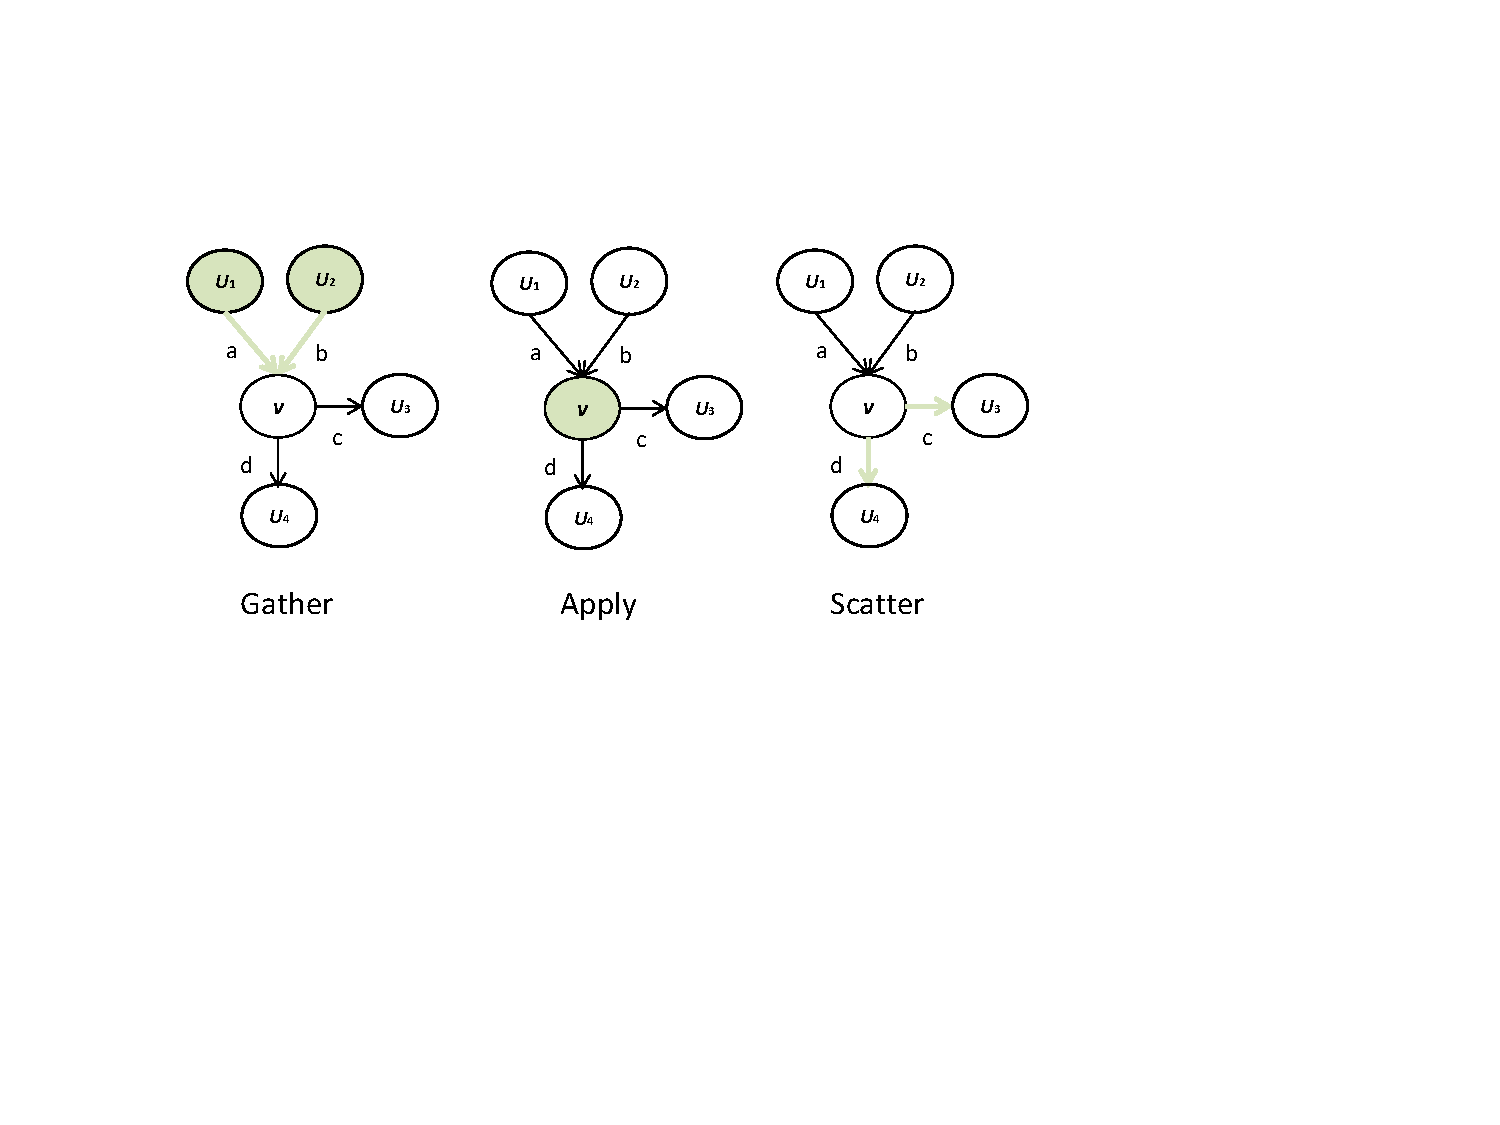
\includegraphics[width=0.9\textwidth,height=\textheight,keepaspectratio]{figures/phases.pdf}
\caption{An example of GAS abstraction. }
\label{fig:phases}
%\vspace{-1\baselineskip}
\end{figure}


GraphReduce exposes the Gather-Apply-Scatter (GAS) computational model used by Pregel \cite{pregel}, Powergraph \cite{powergraph}, and GraphLab \cite{graphlab}.
With GAS, a problem is described as a directed (sparse) graph, $G = (V, E)$, where $V$ denotes the vertex set and $E$ denotes 
the directed edge set. A value is associated with each vertex $v\in V$, and each directed edge $e_{ij}$ is associated with 
a source vertex $u$ and a target vertex $v$: $e_{ij} =(u, v) \in E$. Given a directed edge $e_{ij} = (u, v)$, we refer to 
$e_{ij}$ as vertex $v$'s in-edge, and as vertex $u$'s out-edge. A typical GAS computation, then, has three stages \cite{vertexapi}: 
(1) Initialization, (2) Iterations, and (3) Output. Initialization deals with initializing vertex/edge values and a starting 
{\em computation frontier}, which is defined as the set of active vertices for a given iteration. In each Iteration stage, 
a sequence of iterations is run, each gathering the values seen on the incoming edges, updating the values of elements, and 
then defining a new frontier for the next iteration. Figure \ref{fig:phases} illustrates these three phases, assuming vertex $v$ to be the 
central vertex.


%\vspace{-0.5\baselineskip}
\begin{itemize}
  \item {\bf Gather Phase}: each vertex aggregates values associated with its incoming edges and their source vertices. 
We define the gather function as $G(u, v, e_{ij})$, and we use binary operator $\biguplus$ to aggregate the outputs 
from multiple $G$s into one value $R$. In Figure 1 (a), the result ($R$) from the Gather Phase for vertex $v$ can be represented 
as $R= G(u_1, v, a)\biguplus G(u_2, v, b)$. 
 % \vspace{-0.5\baselineskip}
  \item {\bf Apply Phase}: the value of each vertex in the current frontier is updated through the gather result. 
We define the update function as $U(v, R)$, where $R$ is the result from the Gather Phase. Shown in the Figure 1 (b), 
we have the updated vertex $v$ as: $v' = U(v, R)$.  
 % \vspace{-0.5\baselineskip}
  \item {\bf Scatter Phase}: the new vertex state is propagated to neighbors, by updating the state of its out-edges 
(e.g., $c$ and $d$ in Figure 1). We define the Scatter function for updating the out-edges of $v$ as $S(v', e_{out})$, 
where $v'$ is the updated vertex $v$ and $e_{out}$ represents $v$'s out-edges. Shown in Figure 1 (c), two updated edges 
$c'$ and $d'$ are denoted as: $c' = S(v', c)$ and $d' = S(v', d)$.
%\vspace{-0.5\baselineskip}
\end{itemize} 


As shown in much prior work \cite{powergraph, pregel, sc05}, the GAS model is not only simple to use, but it is also sufficiently general to express
a broad set of graph algorithms, ranging from PageRank to Connected Components, and from Heat Simulation to Sparse Linear Algebra. 
For example, the PageRank algorithm \cite{pagerank} can be expressed as follows. In the {\bf Gather Phase}, each vertex $v_i$ in the current 
frontier accumulates $G_i = \sum_{}^{}{\frac{R_j}{n_j}}$ from all in-edges from source vertex $v_j$, where $R_j$ is the rank of 
$v_j$ and $n_j$ is the number of out-edges ($v_j\rightarrow v_i$) of $v_j$. Then, in the {\bf Apply Phase}, vertex $v_i$ updates 
its value using some common PageRank formula like $R_i = 0.85+0.15\times G_i$. Since in PageRank, the values of out-edges of 	$v_i$ will not change 
in the {\bf Scatter Phase}, there are no operations for this phase. 


\begin{figure}[!t]
\centering
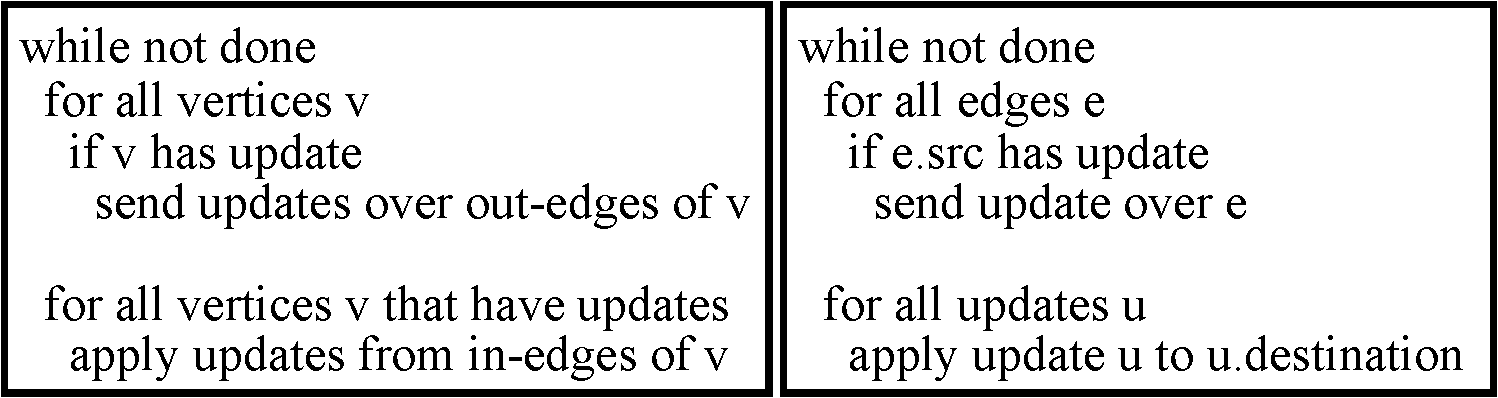
\includegraphics[width=\textwidth,height=\textheight,keepaspectratio]{figures/hybrid-model.pdf}
\caption{ (a) Vertex-centric Scatter-Gather. (b) Edge-centric Scatter-Gather. }
\label{fig:vertex-edge}
%\vspace{-1\baselineskip}
\end{figure}




Figure \ref{fig:vertex-edge} shows two common ways to implement graph algorithms with GAS: edge-centric vs. vertex-centric execution, which differs in whether the
Scatter and Gather phases iterate over and update edges or vertices (their pseudo codes are shown in Figure \ref{fig:vertex-edge}).
Implementation can also vary in terms of Update functions, to be implemented as either Bulk-Synchronous Parallel (BSP) \cite{BSP}
for simplicity or via asynchronous execution, for faster convergence. In either case, the graph algorithm terminates
when some application-specific condition is met, e.g., when no more changes in vertex and edge states beyond a certain threshold. 


\subsection{Motivation and Challenges}




\begin{table}[h]%\scriptsize
\centering
\begin{tabular}{lllc}
Graph Name & Vertices & Edges & \multicolumn{1}{l}{In-memory Size} \\ \hline
\multicolumn{4}{c}{GPU In-Memory} \\ \hline
ak2010\cite{ak2010}& 45,292 & 108,549 & 7.9MB \\
coAuthorsDBLP\cite{coauthors} & 299,067 & 977,676 & 69.5MB \\
kron\_g500-logn20\cite{kron20} & 1,048,576 & 44,620,272 & 2.4GB \\
webbase-1M\cite{web} & 1,000,005 & 3,105,536 & 211.6MB \\
belgium\_osm\cite{belgium} & 1,441,295 & 1,549,970 & 5.4MB \\ \hline
\multicolumn{4}{c}{GPU Out-of-Memory} \\ \hline
kron\_g500-logn21\cite{kron20} & 2,097,152 & 91,042,010 & 4.84GB \\
nlpkkt160\cite{nlpktt} & 8,345,600 & 221,172,512 & 11.9GB \\
uk-2002\cite{uk2002} & 18,520,486 & 298,113,762 & 16.4GB \\
orkut\cite{orkut}& 3,072,441 & 117,185,083 & 6.2GB \\
cage15\cite{cage15} & 5,154,859 & 99,199,551 & 5.4GB
\end{tabular}
\caption{ Datasets used to evaluate GraphReduce framework. `Out-of-memory' means that the input graphs cannot fit into the limited GPU memory. A commercial K20c GPU with a 4.8 GB global memory is used as an example to illustrate in-memory and out-of-memory cases.}
\label{datasets}
%\vspace{-0.5\baselineskip}
\end{table}




\begin{table}[h]%\scriptsize
\centering
\begin{tabular}{cccc}
\hline
Graphs & X-Stream (ms) & CuSha(ms) & \multicolumn{1}{l}{Speedup} \\ \hline
ak2010 & 215.155 & 7.75 & 28x \\
belgium\_osm & 2695.88 & 791.299 & 3x \\
coAuthorsDBLP & 1275 & 11.553 & 110x \\
delaunay\_n13 & 80.89 & 5.184 & 16x \\
kron\_g500-logn20 & 46550.7 & 119.824 & 389x \\
webbase-1M & 3909.12 & 13.515 & 290x
\end{tabular}
\caption{Performance comparision between two state-of-the-art graph processing approaches. X-Stream runs on a 16 core Xeon E5-2670 CPU with 32GB memory. CuSha runs on a NVIDIA K20c Kepler GPU with 4.8 GB memory. }
\label{gpu-cpu}
%\vspace{-0.5\baselineskip}
\end{table}


\subsubsection{Why Graph Analytics Using GPUs ?}
The high compute power and multi-level parallelism provided by the SIMT (Single Instruction Multiple Threads) architectures of GPGPUs \footnote{\scriptsize Without specified mention, NVIDIA terminology will be used throughout the chapter
to illustrate our work. However, the proposed methodology can be easily applied to a wide range of massively
parallel architectures.} present opportunities for 
accelerating many graph algorithms \cite{medusa, cusha,vertexapi,mapgraph}. Table \ref{gpu-cpu} shows the performance comparison between two state-of-the-art graph analytics 
processing the BFS algorithm: X-Stream \cite{xstream} for CPUs and CuSha \cite{cusha} for in-memory GPU processing. Significant performance speedups are
observed from using the GPU. For instance,  graph kron\_g500-logn20 \cite{kron20} processed by CuSha on a commercial K20c Kepler GPU 
(4.8GB memory) achieves 390x speedup over X-Stream on a 16 core Xeon E5-2670 CPU (32 GB memory).

   



%\begin{table}[h]\scriptsize
%\begin{tabular}{lcccc}
%\hline
%Name & \multicolumn{1}{l}{In-Memory GPU} & \multicolumn{1}{l}{CPU} & \multicolumn{1}{l}{Hybrid} & \multicolumn{1}{l}{Static Partition} \\ \hline
%b40c & \cmark &  &  &  \\ 
%Medusha & \cmark &  &  &  \\ 
%MapGraph & \cmark &  &  &  \\
%VertexAPI & \cmark &  &  &  \\ 
%CuSha & \cmark &  &  &  \\ \hline
%GraphChi &  &\cmark  &  &  \\
%X-Stream &  & \cmark &  &  \\ \hline
%Totem &  &  &  \cmark & \cmark \\ 
%GraphReduce &  &  & \cmark  & \xmark\\ \hline
%\end{tabular}
%\caption{\small Features of different graph processing frameworks.}
%\end{table}


\subsubsection{Challenges in GPU Graph Analytics?}
Acceleration of graph analytics via GPUs is limited, however, by the fact that many real-world graphs cannot fit into 
GPUs' limited memories. As mentioned earlier, a common Yahoo-web graph \cite{yahoo} with 1.4 billion vertices requires 6.6 GB memory 
just to store its vertex values. Additional examples of graphs exceeding GPU memory sizes appear in Table \ref{datasets}.
Previous work on GPU-based graph processing has not addressed this issue. CuSha \cite{cusha}, MapGraph \cite{mapgraph}, VertexAPI \cite{vertexapi} and Medusa \cite{medusa} all assume graphs to reside in GPU memory. GraphChi \cite{chi} and X-Stream \cite{xstream} are designed for CPU-based systems, 
unable to benefit from the multi-level massive parallelism offered by GPUs (shown in Table \ref{gpu-cpu}). Hybrid approaches (CPU+GPU) like Totem \cite{totem} are only able to process a fixed sub-graph that can fit into GPU memory after statically partitioning the graph between CPU and GPU, which results in underutilization of GPU's fullest processing power and parallelism. 
 


%Totem \cite{totem} provides a high-level abstraction to address a hybrid environment (CPU+GPUs), 
%by statically partitioning the graphs into GPU and host CPU memories. Specifically, performance improvements are obtained for
%graphs following a power-law vertex distribution by placing low-degree vertices on the CPU and high-degree vertices on the GPU.
%As graph size increases, however, only a fixed sub-graph can fit into GPU memory, leading to diminishing returns for
%such static partitioning, since more and more of the graph processing will be bottlenecked by the slower compute engine (CPU). 




% (\textcolor{red}{/*Figure XX shows examples of large graphs that do not fit in GPU memory and their vertex distributions are not suitable for Totem. I have two graphs of vetex degree %distribution for two large graphs. wait for totem results before adding here /*}). 


\begin{figure}[!t]
\centering
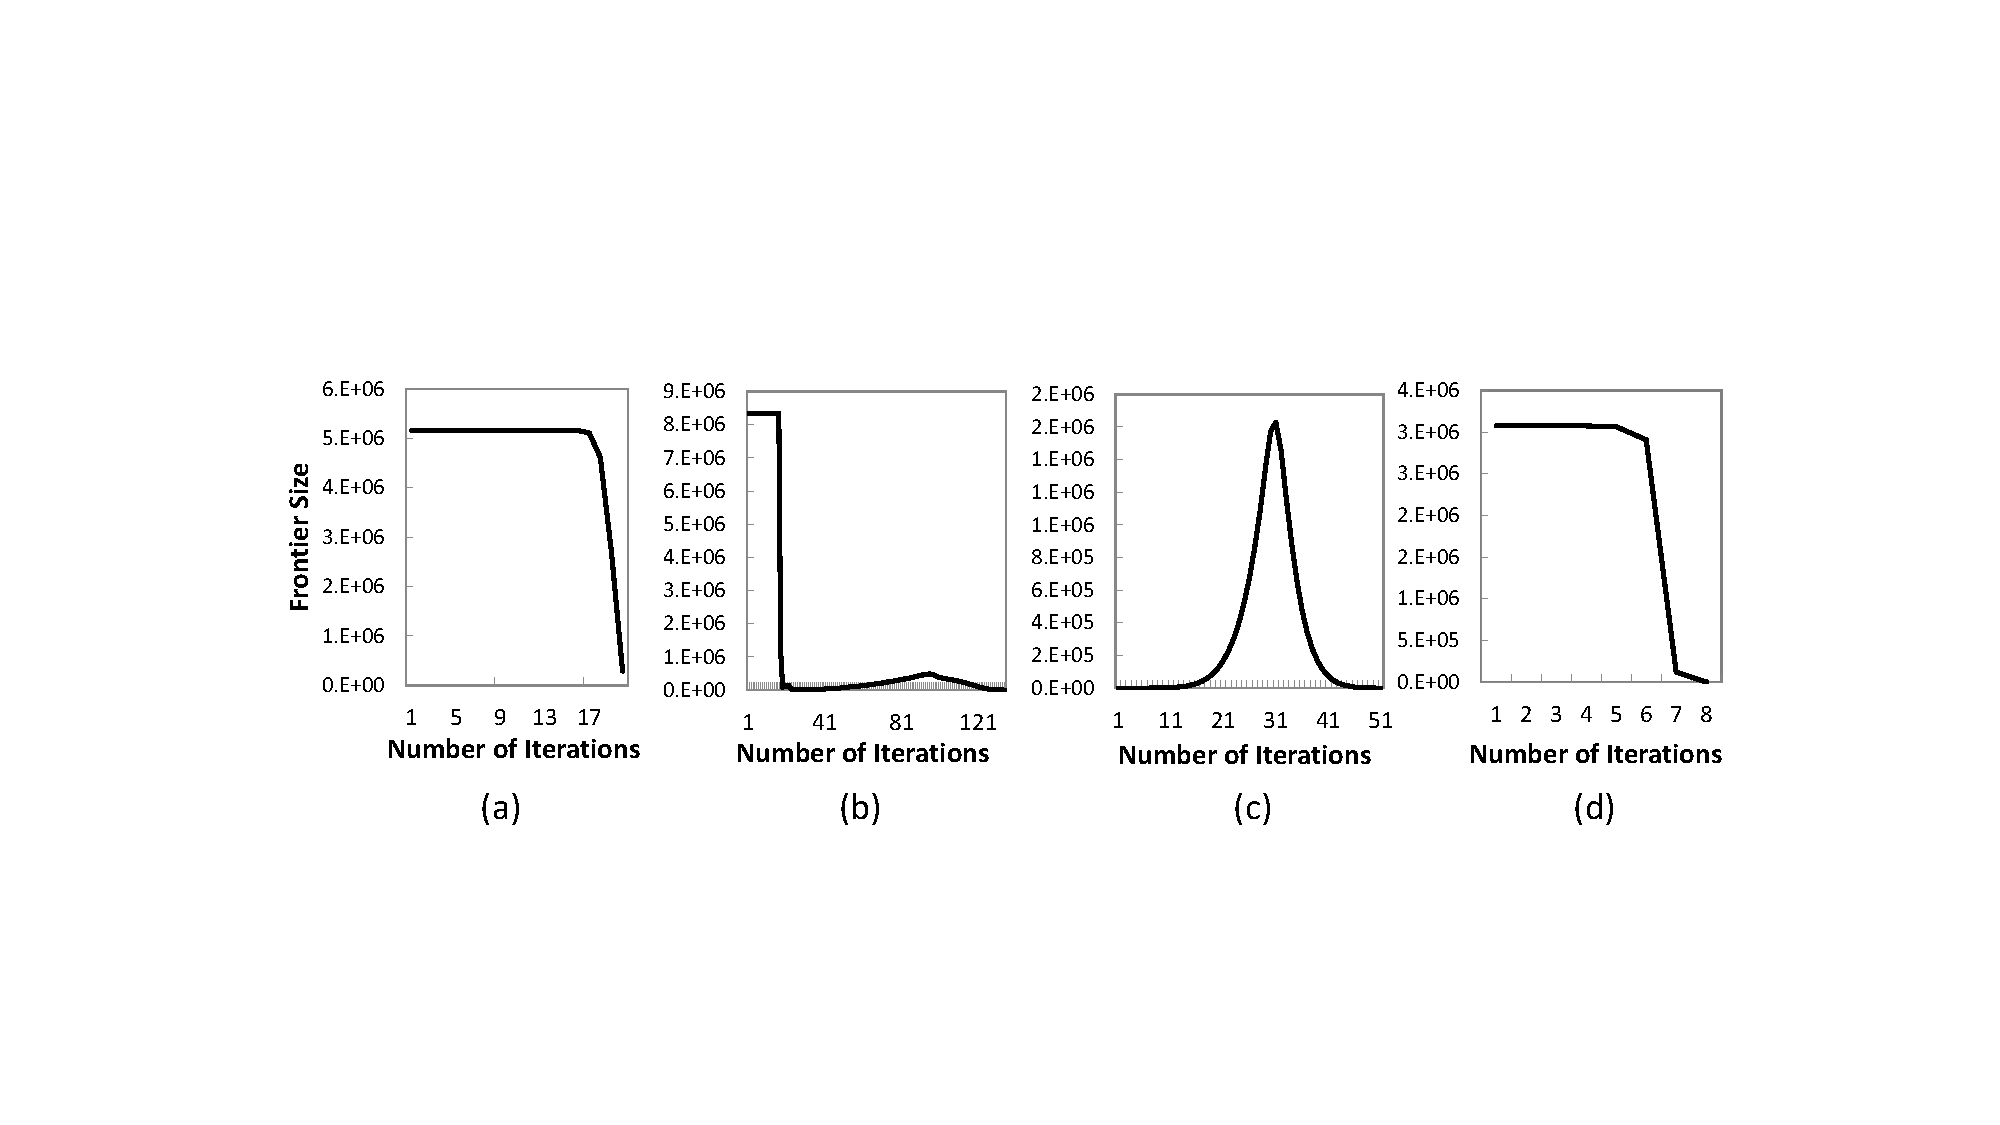
\includegraphics[width=\textwidth,height=\textheight,keepaspectratio]	{figures/frontier.pdf}
\caption{Frontier size changes across iterations using the GAS model on GPUs. This phenomenon highly depends on the input graph and algorithm, showcasing the inherent graph irregularity. Four cases from left to right: (a) Cage15 - PageRank; (b) nlpkkt160 - PageRank; (c) Cage15 - BFS; and (d) orkut - Connected Component (CC). 
 }
\label{fig:frontier}
%\vspace{-0.5\baselineskip}
\end{figure}



There are several challenges to efficiently process larger-than-memory graphs on GPUs. They involve the need to provide end
users with convenient programming constructs for their graph algorithms, but without unduly burdening them with (i) graph partitioning to
fit sub-graphs into GPU memory, (ii) how and when such partitions are moved between GPU and host memories, and (iii) how to best
extract multi-level parallelism from their GPU-resident execution. The GraphReduce framework presented in this chapter 
addresses these challenges.




Graph partitioning or chunking for fitting into GPU memory must deal with the irregular nature of 
graph algorithms and how they access the input data. More specifically, to obtain high on-GPU performance, chunking
must be done to minimize GPU-host data movement. For the GAS model, this requires ensuring GPU memory residence of 
the vertices and edges that actively take part in the computation iterations being performed.
This despite the fact that due to the inherent irregularity in graph algorithms, in every computation iteration, the number 
of edges and vertices that actively take part in computation (computation frontier size) is not constant, and it varies with 
graph algorithms and datasets, as shown in Figure \ref{fig:frontier}. Across all of these cases, the frontier sizes \footnote{\scriptsize The term ``frontier size" is synonymous with the number of active vertices in a given iteration. The variation of the frontier size during execution is sensitive to the starting-point for graph processing. } 
incur significant changes (either dropping or climbing). For instance, in Figure \ref{fig:frontier}(b) for graph nlpkkt160 processed 
by PageRank, the frontier size drops sharply after a few iterations and remains low for the rest of the execution. 
Given these results, ideally, the GR runtime should {\em move sub-graphs to the GPU only if they
contain active vertices and edges}. Otherwise, such movements simply cause unnecessary overhead.
For the same nlpkkt160 case in Figure \ref{fig:frontier}(b), after several iterations, most of the sub-graphs do not have 
active vertices/edges, so there is no need to move those chunks to the GPU. We have found this phenomena to be very common 
across most of the graphs shown in Table \ref{datasets}, for various algorithms. The GR methods presented in this chapter address this issue, along with (ii) and (iii) above.

%%% Design Section

\section{Design Choices}
\label{Choice}

%\vspace{-0.5\baselineskip}

\subsection{Hybrid Programming Model}
\label{3.1}
 
Existing systems choose some specific programming model for graph execution. GraphLab \cite{graphlab}, Pregel \cite{pregel} and GraphChi \cite{chi} use the 
vertex-centric model, while X-Stream \cite{xstream} uses the edge-centric model. In comparison, GraphReduce employs a hybrid programming model
using both edge- and vertex-centric operations. This is because in the GAS model, different processing phases have different 
types of parallelism and consequently, offer different parallelism opportunities, coupled with different memory access characteristics. 
For instance, an edge-centric model should be used in the {\bf Gather Phase} (shown in Figure \ref{fig:phases}), because a GPU hardware thread 
will then be assigned to work on behalf of an edge in the graph. This is preferable to the vertex-centric model, because first,
real-world graphs commonly have more edges than vertices (shown in Table \ref{datasets}), thus giving rise to higher degrees of
parallelism and decreased GPU core idling. Second, in the vertex-centric approach, each vertex receives information from multiple in-edges, 
resulting in a consequent need for synchronization or atomics to order the receive operations from each of the in-edges. This could potentially degrade 
the overall performance. The same observations hold for using the edge-centric model in the {\bf Scatter Phase}. In contrast, 
in the {\bf Apply Phase}, there are parallelism opportunities only over the vertex set, thus favoring a vertex-centric model.

%\vspace{-0.5\baselineskip}
\subsection{Characterization of Buffers in Play}
\label{3.1}

\begin{figure}[!t]
\centering
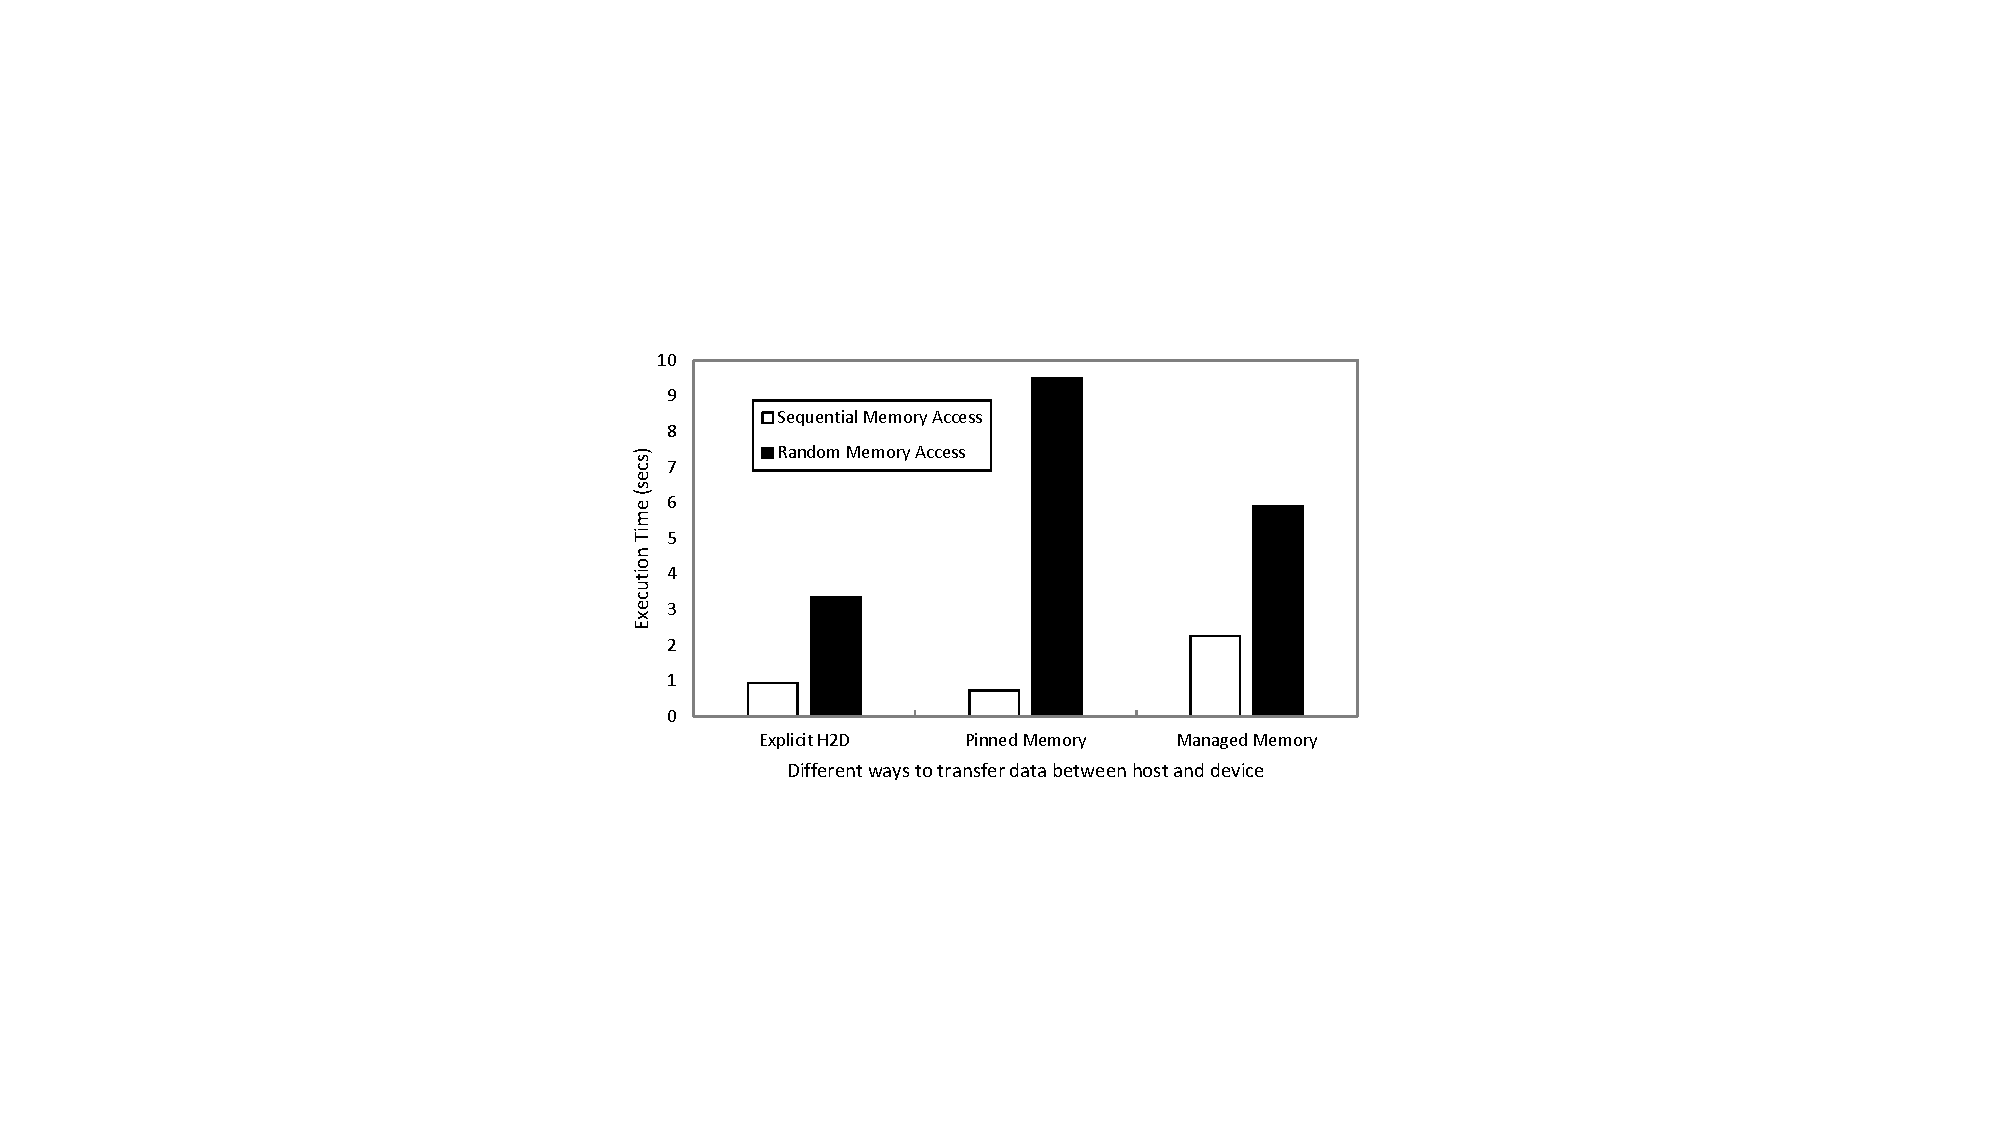
\includegraphics[width=0.75\textwidth,height=\textheight,keepaspectratio]{figures/transfer.pdf}
\caption{Performance of transferring 100,000,000 double elements, using three techniques for data exchange between CPU and GPU.  }
\label{fig:transfer}
%\vspace{-1\baselineskip}
\end{figure}

\begin{figure}[!t]
\centering
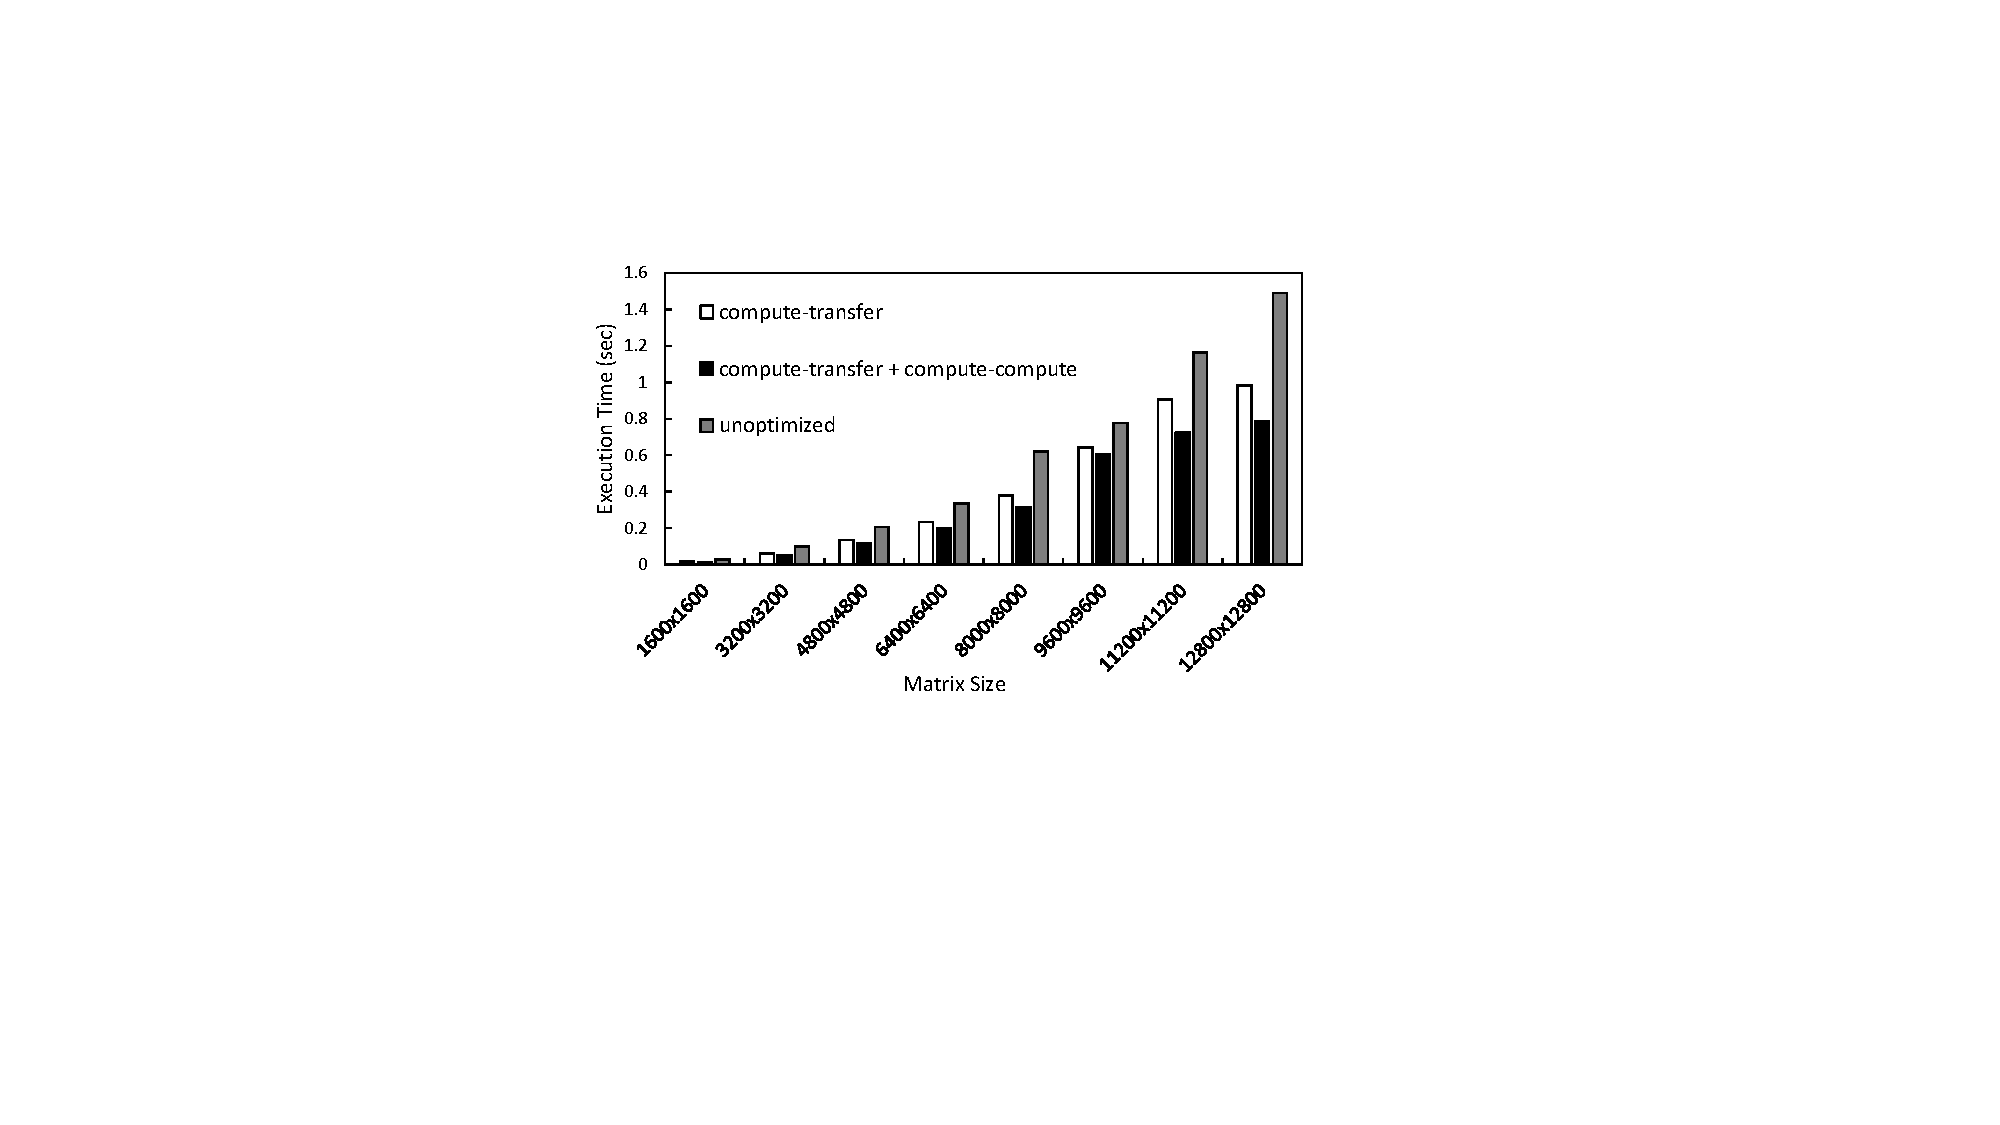
\includegraphics[width=0.75\textwidth,height=\textheight,keepaspectratio]{figures/2schemes.pdf}
\caption{Performance benefits of using a combination of compute-transfer and compute-compute schemes for processing matrix multiplication with different input sizes. Stripe size=50, which refers to the contiguous number of rows of the matrix being fetched into the GPU memory as a chunk.  }
\label{fig:2schemes}
%\vspace{-0.5\baselineskip}
\end{figure}

Graph data chunked to fit into GPU memory and to be moved from host to GPU, is comprised of edges that have either a destination or 
a source vertex in some well-defined graph partition (see Section 3.3.2 for details). Henceforth termed {\em shards}, such chunks reside
in memory buffers that experience different access patterns. GraphReduce characterizes such access patterns in order to appropriately map
corresponding memory buffers to the memory abstractions exposed by current GPUs. In terms of data movement, buffers can be classified as static 
vs. streaming buffers. Static buffers are copied only once to GPU memory, typically in the Initialization phase. They remain there for 
the lifetime of the graph execution. An example is a vertex set of a graph that fits into GPU memory. Streaming buffers, on the other
hand, are moved in and out of GPU memory as processing progresses, and at any point in time, a particular instance of some streaming buffer 
resides in GPU memory, e.g., a subset of a graph's edge set. In the GAS programming model, static buffers are accessed in all three phases, 
while streaming buffers only appear in a single phase. Another way to characterize buffers is by their access rules, such as read-only 
or read/write access. For example, vertex and edge data buffers (containing mutable states) have both read and write access patterns, 
while the vertex set (containing immutable vertex IDs) is read-only. Based on these attributes, the GR runtime makes decisions on whether 
or not to transfer certain buffers back to the host (see Section 3.3.3). Finally, buffers can be classified in terms of the spatial locality 
of their accesses, e.g., random or sequential access. For example, in the edge-centric approach shown in Figure \ref{fig:vertex-edge}, 
there are random accesses to the vertex set.

Once characterized, buffers are mapped to the different memory abstractions exposed by GPU, which at minimum, contain slow and fast memory~\cite{nemu} 
(e.g., host memory and GPU memory). In the different phases of the GAS model, there are a mix of random and sequential accesses to the input 
buffers (e.g., edge/vertex sets). For this mix, we posit that random access to slow memory is much more expensive than random access 
to faster memory, whereas for sequential access, memory-level parallelism and prefetching can help mask slower memory access speed. Therefore, due to the limited fast memory size (GPU), we choose to map all sequential accesses in a GAS phase to the slower CPU memory and all the random accesses to the faster GPU memory. 
We next validate these assumptions.

Figure \ref{fig:transfer} depicts the performance of three techniques for data exchange between host and GPU (through CUDA runtime APIs): 
(a) explicit data transfer using cudaMemcpy() or \textit{Explicit H2D}; (b) \textit {Pinned Memory} using Unified Virtual Addressing (UVA) \cite{UVA}, 
in which data is transferred implicitly by the CUDA runtime but the memory is allocated as locked memory on the host side; and 
(c) \textit {Managed Memory} (introduced in CUDA 6 \cite{UVA} as Unified memory), where data is transferred between host and device on demand. 
The measurements shown in the figure illustrate that in the case of sequential memory access, \textit{Pinned Memory} performs the best, 
because the accesses directly translate to memory loads/stores operations over the PCIe in which (i) sequential accesses benefit from 
memory level parallelism (MLP) and (ii) software-level prefetching can hide communication overheads. In the case of random access, 
\textit{Explicit H2D} performs the best and \textit{Pinned Memory} performs the worst. In other words, random access performs 
best when data resides in faster GPU memory, and the performance of the \textit{Pinned Memory} degrades as the load/store memory operations 
over the PCIe fail to benefit from prefetching (after all, accesses are random!). Since \textit{Pinned Memory} performs the best 
for sequential accesses, one straightforward approach is to organize graphs such that all memory accesses are sequential. 
However, because of the significant number of random accesses to either the edges or vertices of a graph in at least one phase of the 
GAS model \cite{chi,xstream}, this is not a viable solution for GR as the benefits of sequential accesses  are overshadowed by the huge overhead of the random accesses to the slow memory. In response, GR uses explicit data transfer as the mechanism for transferring 
data between host and device, in way that aim to leverage GPU memory coalescing and software prefetching for the sequential accesses. Although certain performance benefits may exist through intellegent runtime buffer-type selecting. we leave this exploration for the future work. 

\subsection{Coordinated Computation and Data Movement}

The spatial choice of where in memory to locate data requires an associated temporal choice in when to perform data movement
between host and GPU memories. GR uses two methods to attain high performance: (1) hide communication costs by overlapping 
GPU computation with necessary data transfers, and (2) utilize the GPU's inherent high degree of potential internal parallelism. 
(1) is obtained via software-based prefetching to move shards into GPU memory while GPU kernel(s) are being executed. 
(2) is realized by leveraging underutilized GPU resources (idle threads) caused by the irregular nature of graph processing (shown in Figure~\ref{fig:frontier}).
It involves (i) detecting such idle threads, using the computation frontier information available to the GR runtime, and (ii) initiating the
execution of new shards when idleness is present (note that shards within a single GAS phase do not have data dependencies, so they can
be processed in parallel). GR accomplishes this by automatically launching multiple kernels (within the same context), according to the resources
available in each GAS phase. Denoting (1) as {\em compute-transfer} scheme and (2) as a {\em compute-compute} scheme,
Figure~\ref{fig:2schemes} shows the performance benefits obtained from using these approaches vs. an unoptimized scenario when processing a large matrix that 
doesn't fit into GPU memory, thus clearly demonstrating the importance of coordinating
computation with data movement. We will use these two schemes for processing graph algorithms across phases in the GAS model. 
% We will have detailed analysis in the experiment section.

\section{GraphReduce Framework}
\label{Arch}




The GraphReduce framework can efficiently process graphs with large inputs and mutable edge values 
that cannot fit into the limited memories of discrete accelerators. GraphReduce simplifies graph analytics 
programming by supporting a multi-level, asynchronous model of computation. Figure \ref{fig:big1} shows the general 
software architecture of GraphReduce which consists of three major components: Partition Engine, 
Data Movement Engine, and Compute Engine, all supporting an easily used GAS-based API.


\begin{figure}[!t]
\centering
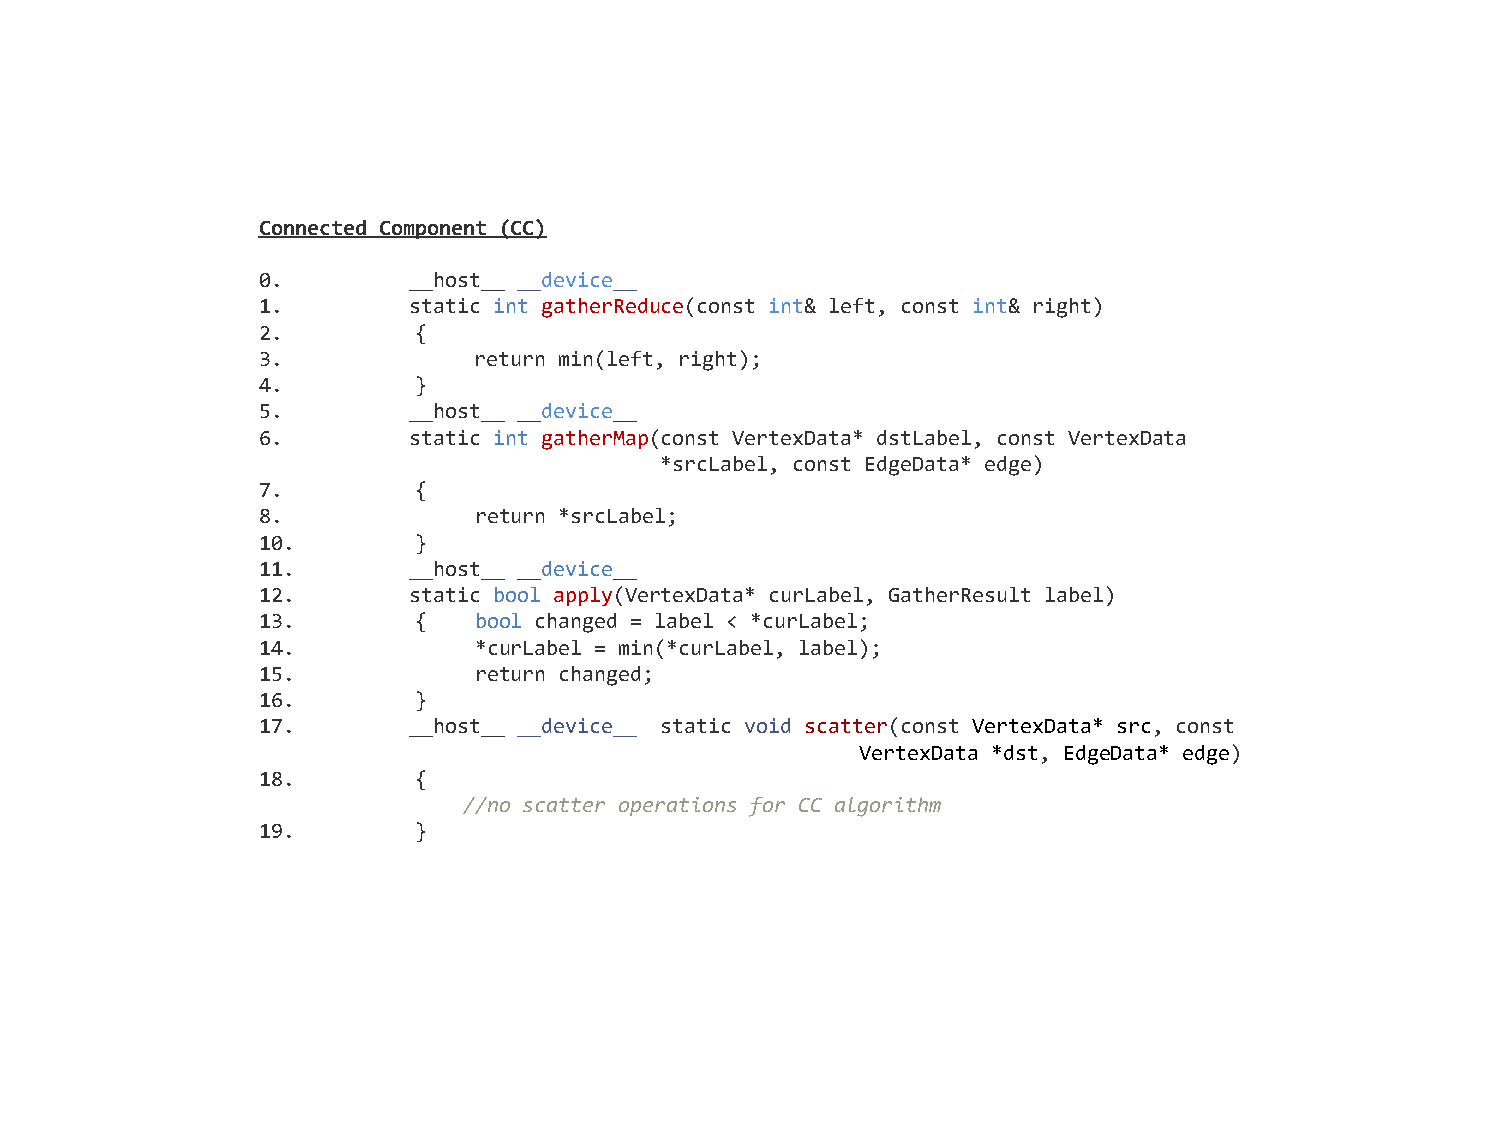
\includegraphics[width=\textwidth,height=\textheight,keepaspectratio]{figures/CC_code.pdf}
\caption{Writing sequential code using GAS model for Connected Component (CC) algorithm in GraphReduce. }
\label{fig:seq}
%\vspace{-1\baselineskip}
\end{figure}


\begin{figure}[!t]
\centering
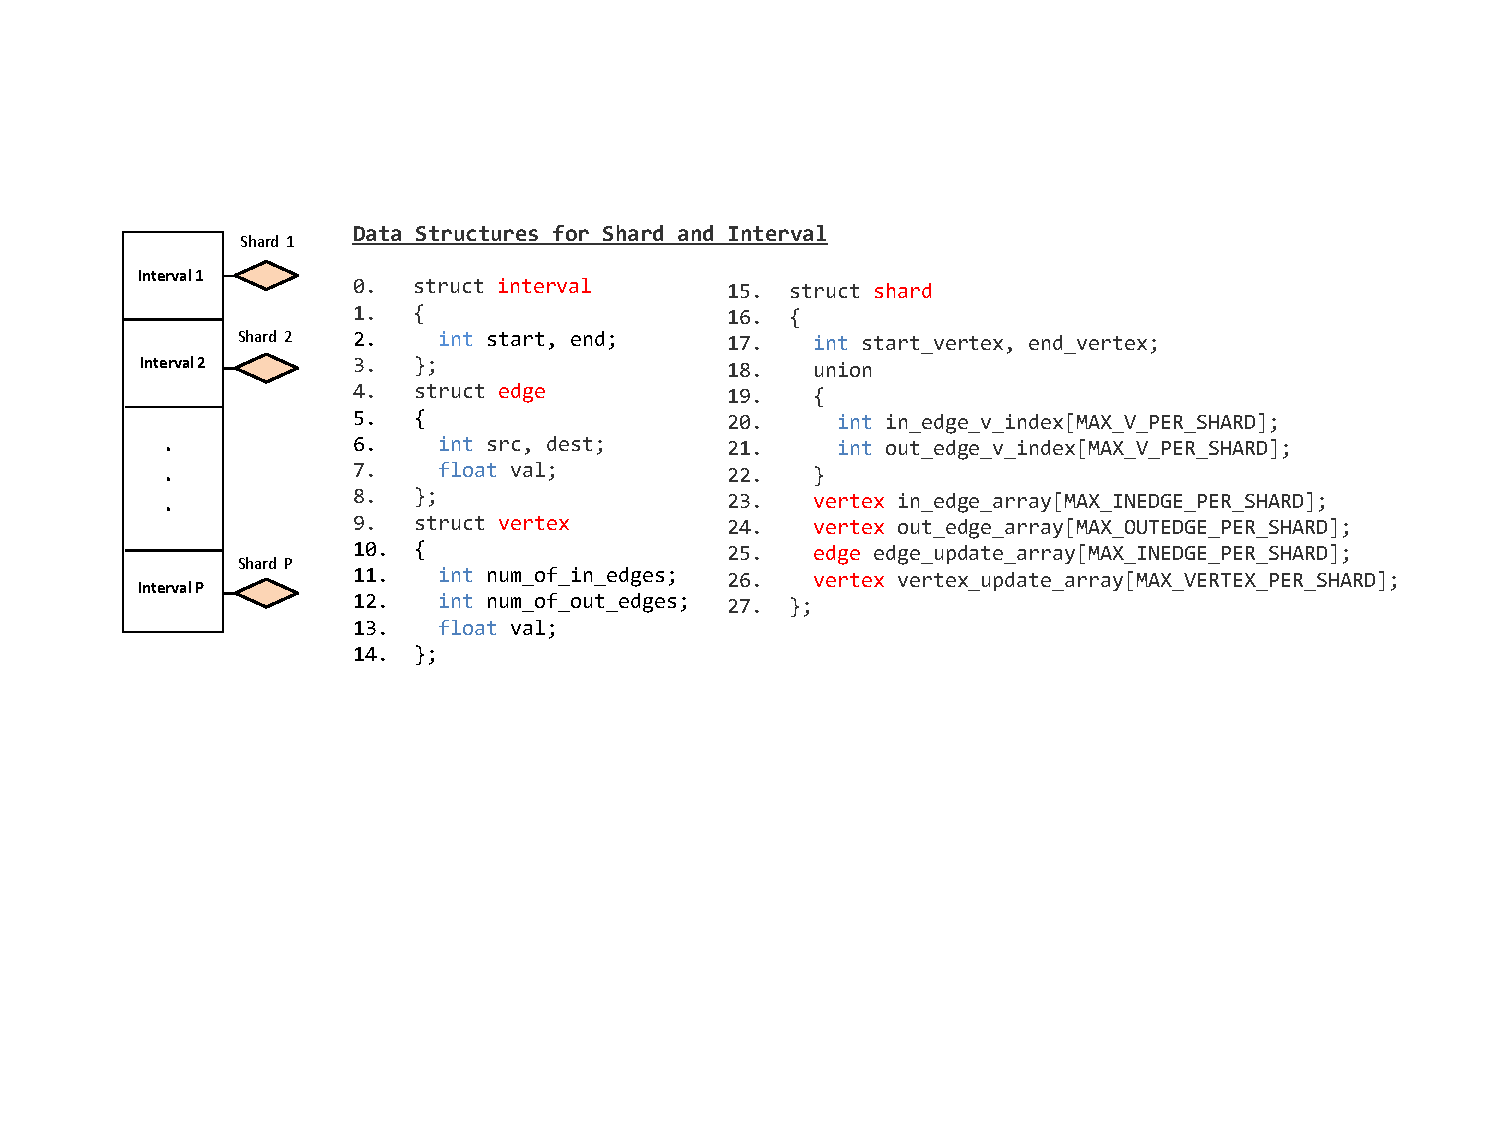
\includegraphics[width=\textwidth,height=\textheight,keepaspectratio]{figures/shard.pdf}
\caption{Illustration of \textit{shard} and its data structure. }
\label{fig:shard}
%\vspace{-0.5\baselineskip}
\end{figure}




\subsection{User Interface}
\label{interface}


As shown in Figure \ref{fig:seq}, programmers can write a sequential algorithm by simply defining the graph's state data types 
(for vertices and edges) and four functions for the different phases in the GAS programming model. 
GraphReduce will then seamlessly generate parallel codes to run on the GPU. User-defined functions 
include $gatherMap()$, $gatherReduce()$, $apply()$ and $scatter ()$, corresponding to the functions defined in Section 3.1.1,
i.e., to $G()$, $\biguplus$, $U()$, and $S()$. Along with the vertex and edge data types, these functions are stored in a tuple 
called UserInfoTuple: $<$$gather()$, $apply()$, $scatter()$, $VertexDataType$, $EdgeDataType$$>$.



%\vspace{-0.5\baselineskip}



\subsection{Partition Engine}
\label{partition}



\begin{figure}[!t]
\centering
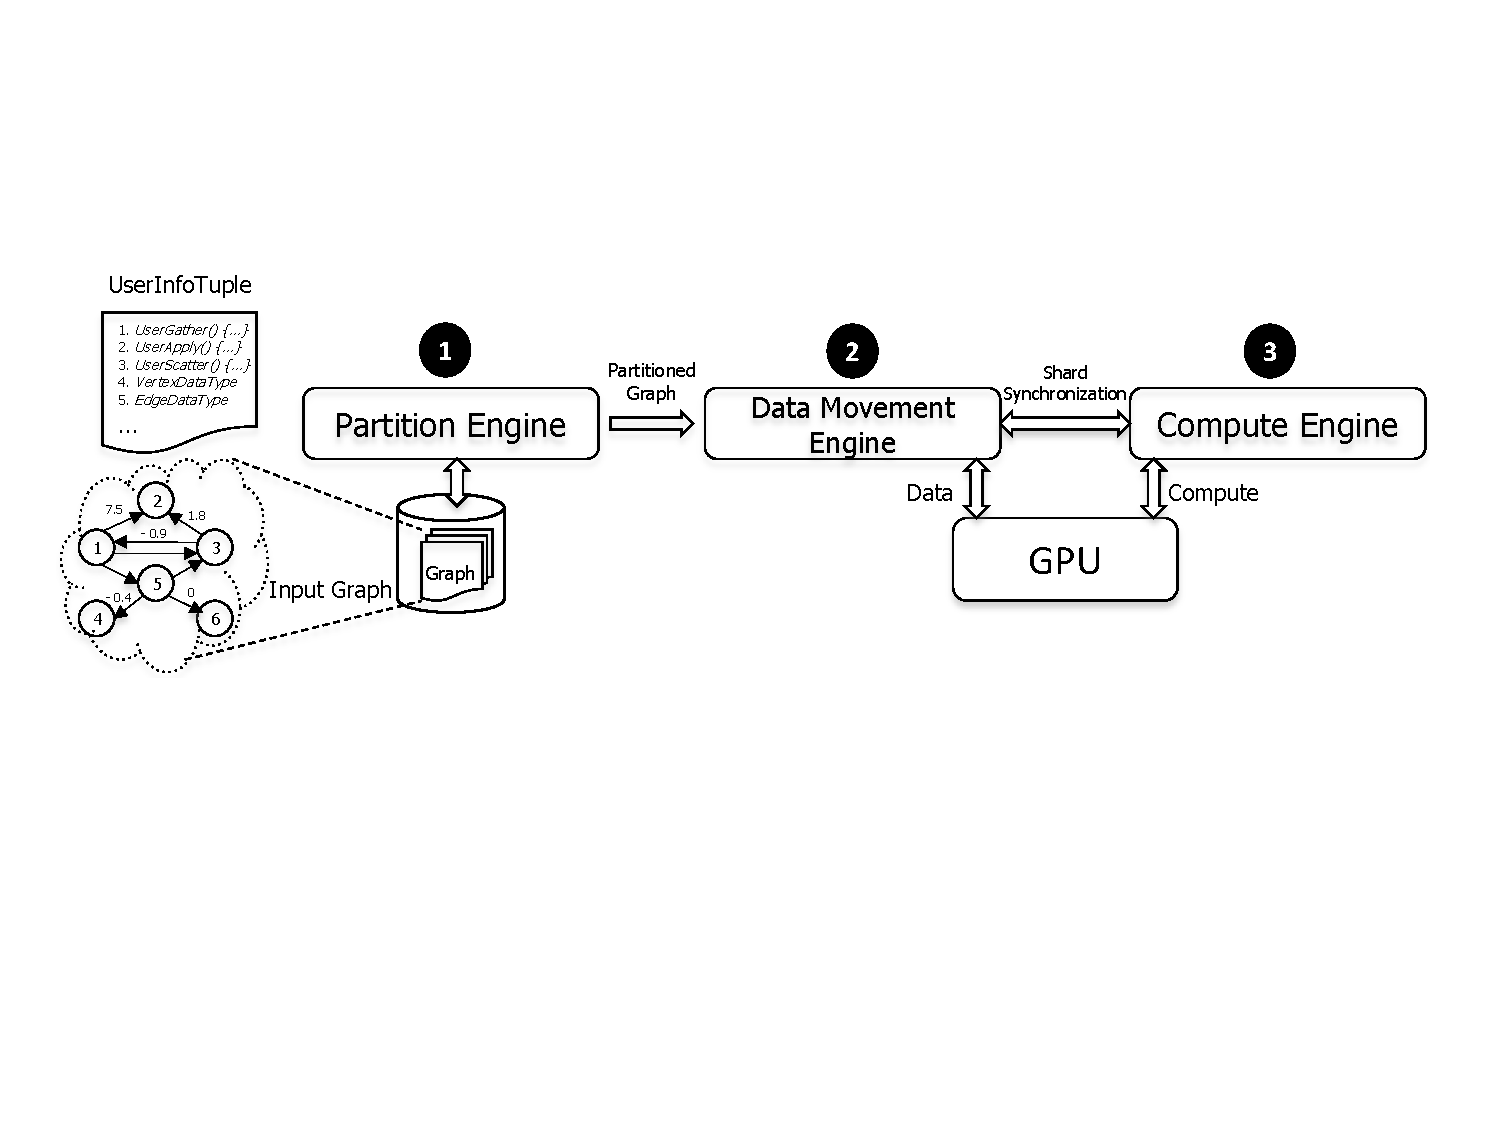
\includegraphics[width=\textwidth,height=\textheight,keepaspectratio]{figures/big1.pdf}
\caption{Architecture of GraphReduce framework. }
\label{fig:big1}
%\vspace{-1\baselineskip}
\end{figure}




%Figure \ref{fig:big2} shows the structure of the Partition Engine. 



The \textit{Partition Engine} shown as \textbf{1} in Figure \ref{fig:big2} is responsible for (1) load-balanced shard creation and (2) providing graph partitioning logics and 
associated orderings of vertices/edges. Partitioning is performed by dividing the vertex set $V$ of graph $G = (V, E)$ into 
disjoint intervals (i.e., sets of vertices) and for each interval, maintaining a \textit{shard} data structure 
(shown in Figure \ref{fig:shard}), where each shard stores all of the edges that have either a destination or a source vertex 
in that interval.

%, so that their union is the entire edge set of the input graph.
% intervals are ranges in the vertex set, and shard represent the set of edges that has source and destination vertices in a particular interval. So for a particular interval there is an %associated shard. Chunks and shards have been used interchangebly in the chapter.

GraphReduce answers the following questions about such sharding: (1) choice of interval, (2) number and sizes of shards,
and, (3) how to order the edges in each shard. For (1), shown in Figure \ref{fig:shard}, %dipanjan...note the 'x' here
intervals are chosen by the Shard Creator of the Partition Engine in a load-balanced fashion. Specifically, each shard contains an approximately 
equal number of edges (in- plus out-edges). %dipanjan....want to say anything more about the actual algorithm being used...at least a citation to something similar?
For (2), the number of intervals P is chosen such that at least one shard (maybe multiple) can be loaded completely into 
GPU memory. Therefore, if more than one shard is allocated in GPU memory, the total number of shards simultaneously participating in graph computation can be calculated as a function of the total number of concurrent memory copy operations to and from the GPU. %dipanjan...please check..you had said something slightly different, but I could not understand it
 Finally, for (3), the graph dataset is a set of source and destination vertex pairs (edges) with the associated value for each edge.
This set of tuples is generally unordered. The Graph Layout Engine inside of the Partition Engine defines the layout of the data by sorting %dipanjan...note the xxx here
the in-edges in the order of their destinations and the out-edges in the order of their sources. 
For such sorted data, we use the compressed Sparse Column (CSC) and compressed Sparse Row (CSR) formats \cite{csr} to store graphs 
to be used in the Gather and Scatter phases, respectively. Therefore, there is no overhead for runtime data-format transposition between CSC and CSR formats.

Edges are stored in some specific sorted order for three reasons. First, with ordered edges, the data moved across the 
PCIe link from host to GPU is contiguous, which can improve system throughput. Second, when updates are collected 
for each vertex in the gather phase, they can be stored in consecutive memory locations for each vertex, which avoids random memory 
accesses. Similarly, the out-edges are stored in the order of source vertices, so that the neighbors of a vertex whose states 
have been updated can be accessed sequentially. Third, sequential accesses to GPU memory can improve performance due 
to memory coalescing. Note that although we are sorting the source and destination vertices when partitioning graphs, GraphReduce is able to take any user-provided partitioning logic as a plug-in to the \textit{Partition Logic Table} inside the Partition Engine (Figure \ref{fig:big2}). 

%\vspace{-0.5\baselineskip}


\begin{algorithm}[htp]
{%\scriptsize
\caption{\footnotesize \label{asynchronous} Asynchronous Memory Copy and Computation for Processing Shards on GPU} 
\label{alg1}
\begin{algorithmic}[1]
\STATE{{\bf MemcpyAsync\_Host2Device (stream\_id)};}

/*{Multiple Streams work on several shards from different intervals simultaneously}*/
\STATE{{\bf GPU\_Computation\_Task(stream\_id)};}

/*{Computation on GPU will not start until a complete shard is available in the memory}*/
\STATE{{\bf MemcpyAsync\_Device2Host (stream\_id)};}

\end{algorithmic}
}
\end{algorithm}



\begin{figure}[!t]
\centering
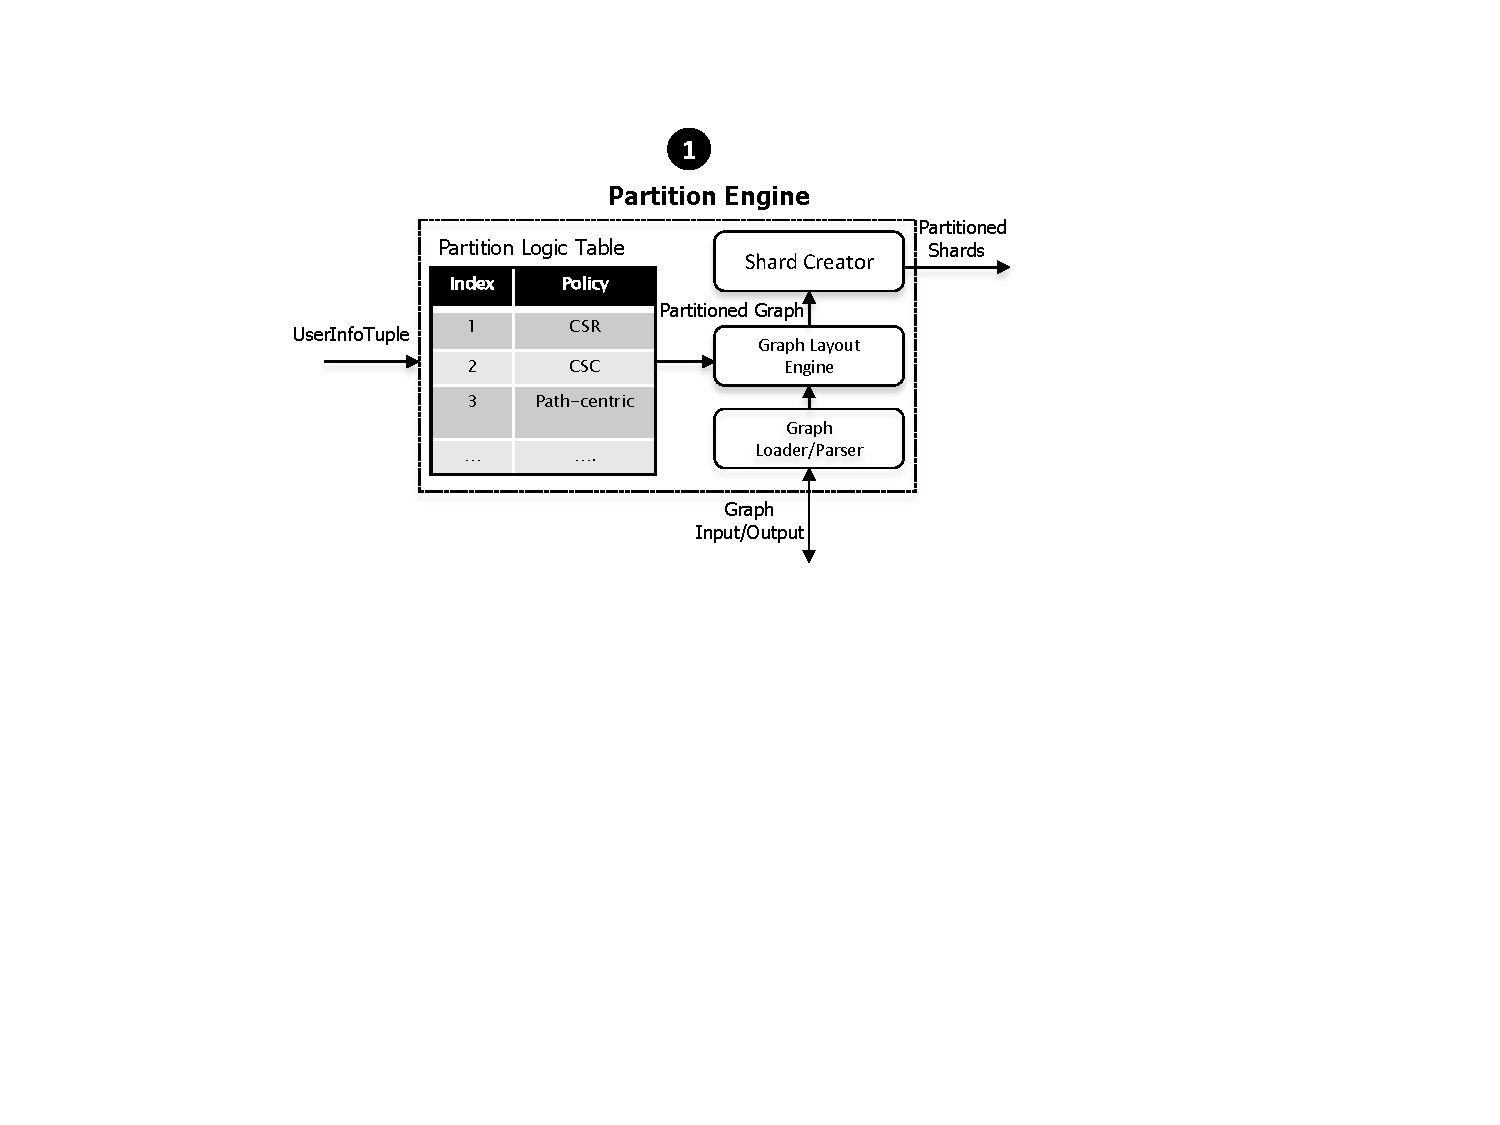
\includegraphics[width=0.75\textwidth,height=0.75\textheight,keepaspectratio]{figures/big2.pdf}
\caption{ The structure of the Partition Engine.}
\label{fig:big2}
%\vspace{-1\baselineskip}
\end{figure}


\begin{figure*}[t]
\centering
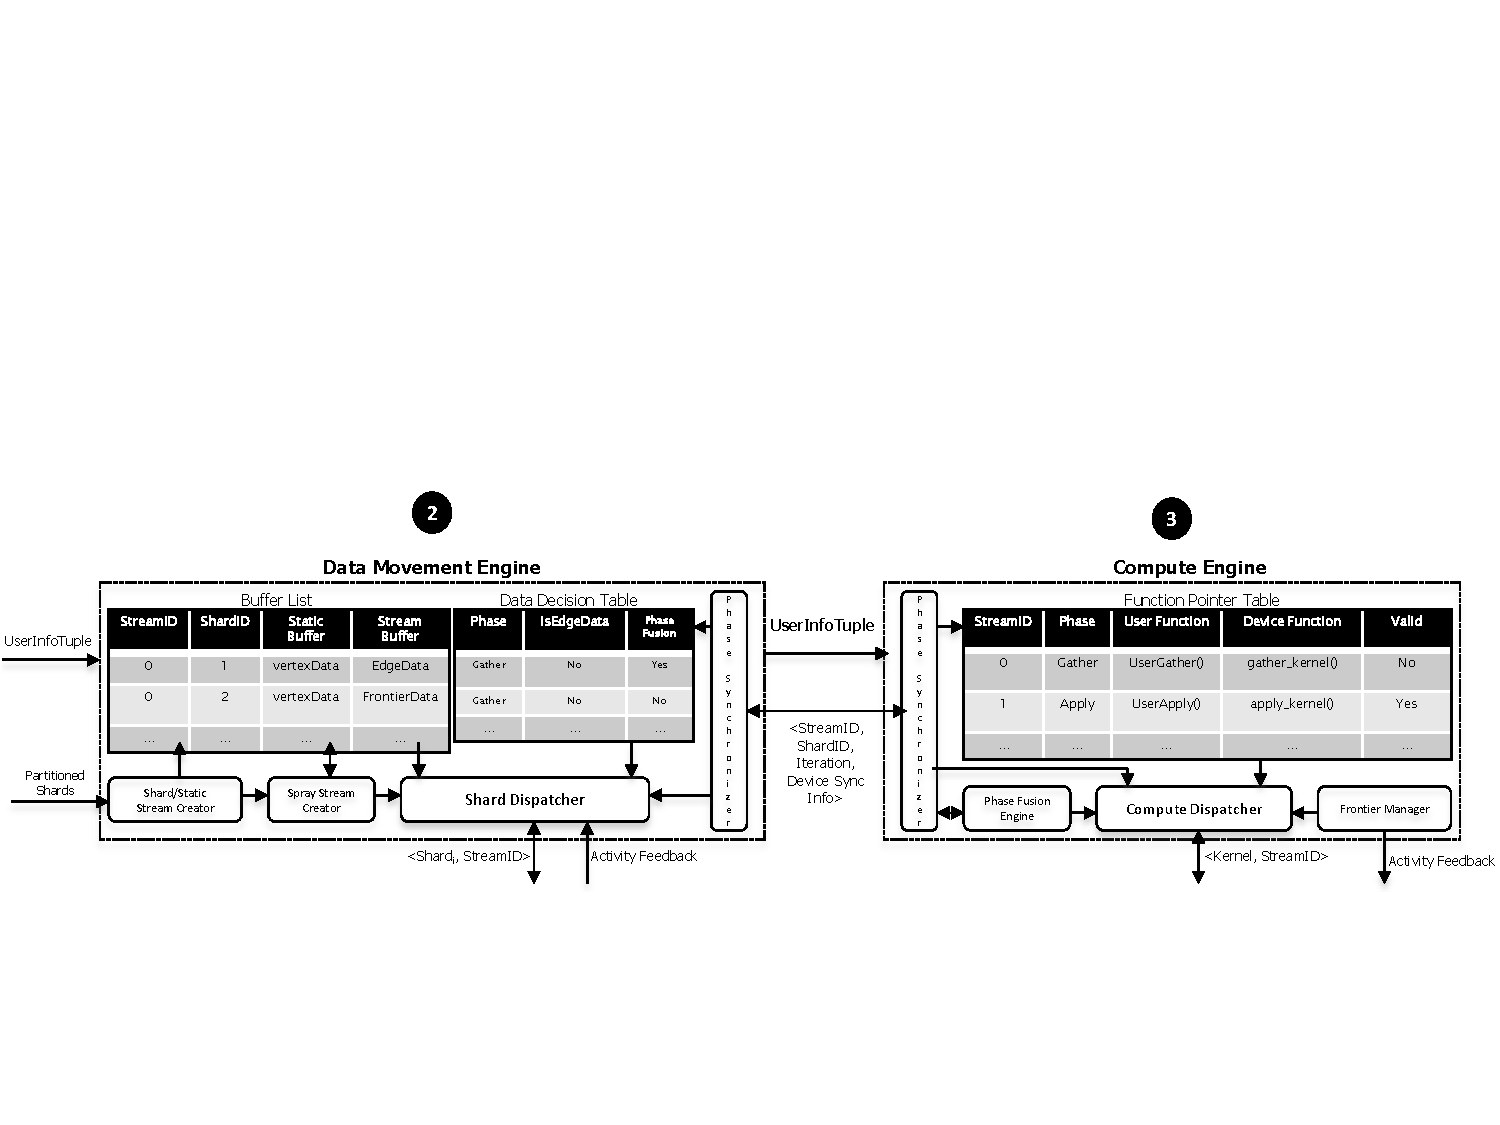
\includegraphics[width=\textwidth,height=\textheight,keepaspectratio]{figures/big_new.pdf}
\caption{ The structures of the Data Movement Engine and Compute Engine. Tables/buffer\_list are data structures (passive elements of the engine) while rectangles are modules (active elements of the engine).}
\label{fig:big_new}
%\vspace{-1\baselineskip}
\end{figure*}


\subsection{Data Movement Engine}
\label{movement}


To address the cost of data movement caused by accesses to and updates of edge/vertex states, the Data Movement Engine 
(shown in Figure \ref{fig:big_new} as \textbf{2}) in GraphReduce seeks to accelerate data movement via asynchronous memory-copy operations for concurrent GPU kernel execution. For instance, for NVIDIA GPUs, the programming environment 
allows the concurrent execution of operations from the same GPU protection domain or context. A sequence of operations 
that execute in issue-order on the GPU is defined as a \textit{Stream Object} \cite{cuda7}. Operations from multiple \textit{Streams} 
can be executed concurrently and interleaved, leveraging the parallelism provided by multiple hardware queues (e.g., Hyper-Qs \cite{kepler}
provided by NVIDIA Kepler architectures shown in Figure \ref{fig:hyperq}(a); they permit host to launch multiple concurrent 
kernels onto a single GPU). In GraphReduce, multiple intervals (and their associated shards from the Partition Engine) can also be 
concurrently processed by different \textit{Streams}, to obtain a high degree of parallelism. For different shards,
each \textit{Stream} spawned by the \textit{Static Stream Creator} inside the Data Movement Engine in Figure \ref{fig:big_new} typically issues multiple MemcpyAsync() 
operations and graph computation kernels asynchronously, overlapping data transfer with computation time. In the Data Movement Engine, 
\textit{Streams} are scheduled and ordered, with the goal to maximize concurrency in data transfer and computation 
across different shards of the graph. 

We now show how to derive the optimal number of shards being transferred concurrently, to maximize the use of PCIe bandwidth. 
Assuming that shard size is sufficiently large to saturate PCIe bandwidth (since we are dealing with large graphs),
we determine the optimal number of shards transferred concurrently as a function of concurrency (number of concurrent operations). 
Specifically, we define $P$ as the total number of shards, $G$ as the size of the entire graph including vertices and edges, 
$V$ as the size of the vertex set, $E$ as the size of the edge set, $K$ as the total number of concurrent \textit{Streams}; 
$M$ as the GPU memory size; and $B$ as the bytes needed to achieve maximum PCIe bandwidth. We will have: 


\vspace{-6pt}
{%\scriptsize
\begin{equation}
\label{equ:shard1}
K*(V/P) + K*B \leq M 
\end{equation}}

\vspace{-14pt}
{%\scriptsize
\begin{equation}
\label{equ:shard2}
B =|(\alpha \times |E|+\beta \times |V|)   
\end{equation}}

%\vspace{-0.5\baselineskip}

where the upper bound of $K$ depends on the GPU architecture (e.g., $K\leq 32$ in K20 NVIDIA GPUs), and $\alpha$ and $\beta$ 
are the number of edge- and vertex-set streaming buffers (discussed in Section 3.2.2) used in each Stream. In Equation (\ref{equ:shard1}), $V/P$ is the size of the interval of the vertex set for one partition. $B$ is the minimum buffer size to saturate PCIe bandwidth (we assume each shard is big enough to saturate that bandwidth). Unknown parameters are $K$ and $P$, of which $P$ can be derived from fixing the shard size to maximum PCIe bandwidth (Equation (\ref{equ:shard2})). With the limited GPU memory size $M$, the maximum number of concurrent transfers is bounded by the size of vertex interval plus the sizes of concurrent shards. For instance, based 
on (\ref{equ:shard1}) and (\ref{equ:shard2}), we can estimate the optimal number of shards being transferred concurrently to be 
$2$ for our NVIDIA K20 Kepler GPU with 4.8 GB memory.


%\vspace{-0.5\baselineskip}



\subsection{Computation Engine}
\label{computation}


The \textit{Computation Engine} shown as \textbf{3} in Figure \ref{fig:big_new} is mainly responsible for GPU in-memory computation (i.e., parallelize each 
phase of the GAS model) and to send feedback information to the \textit{Data Movement Engine} about the computation frontier 
used for the next iteration (discussed in Section 3.1.2) .

%\iffalse
\begin{figure}[!t]
\centering
%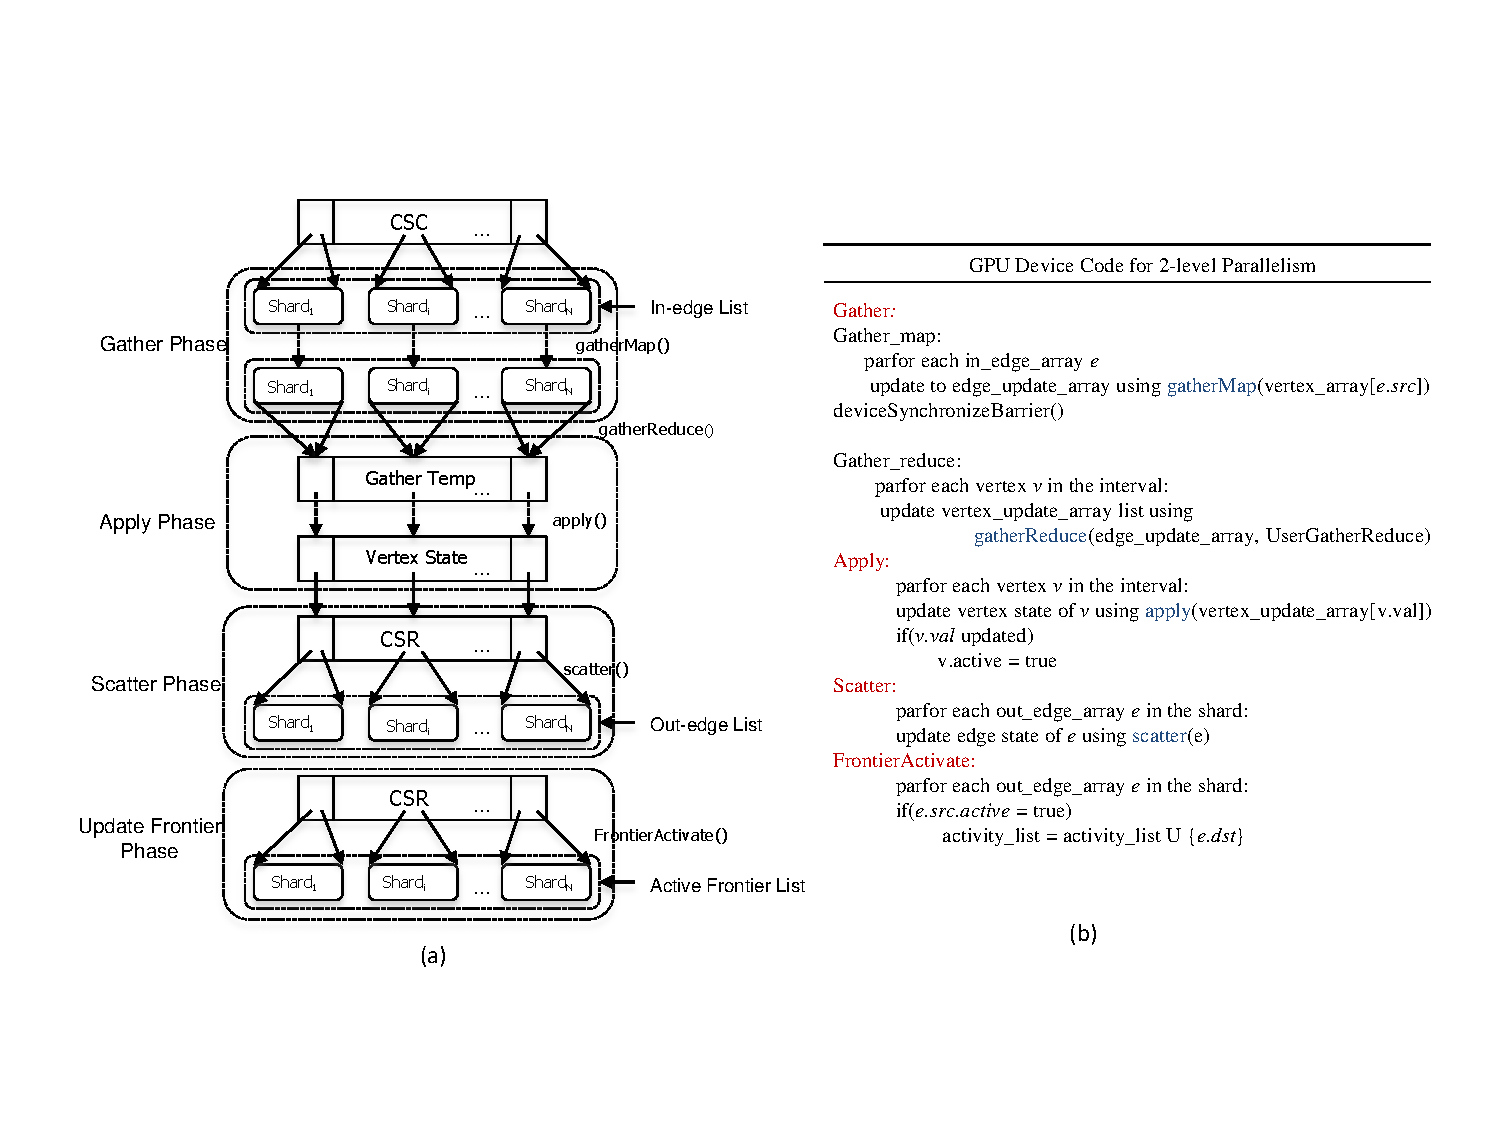
\includegraphics[width=\textwidth,height=\textheight,keepaspectratio]{figures/5phases_1.pdf}
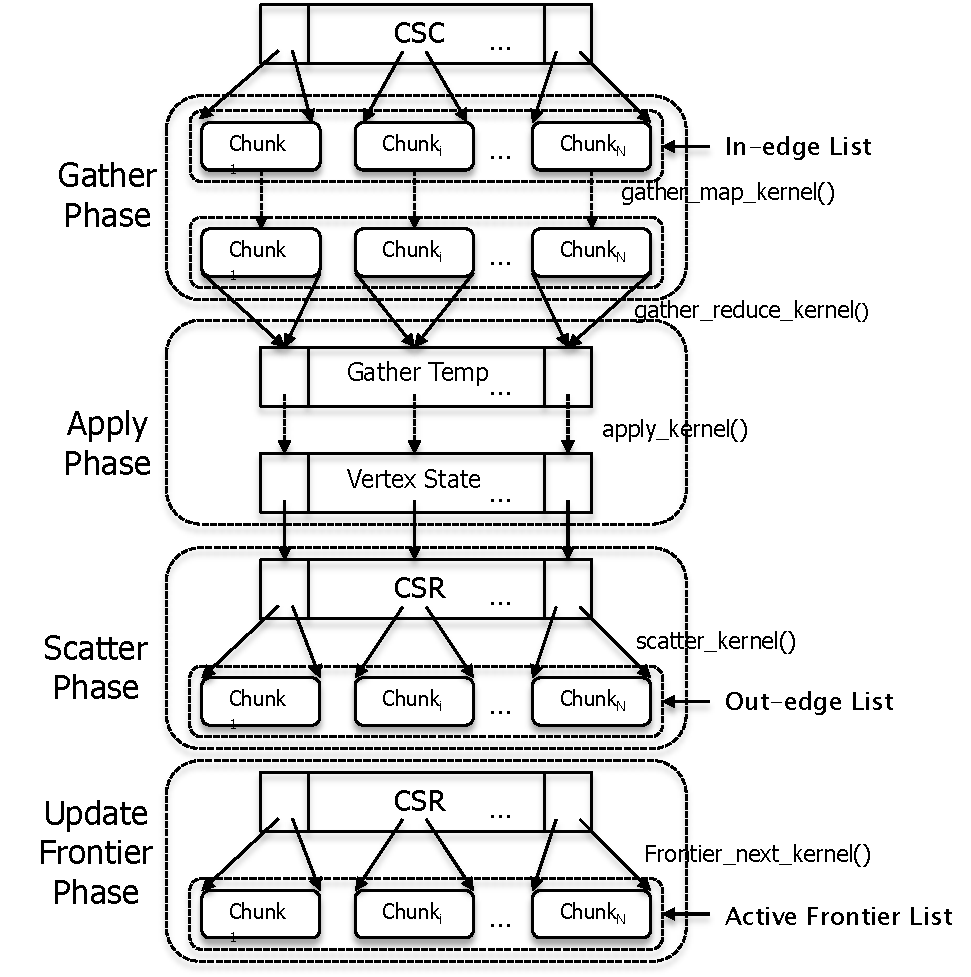
\includegraphics[width=0.85\textwidth,height=\textheight,keepaspectratio]{figures/fivephases.pdf}
\caption{Sub-phases of  the computation stage.  }
\label{fig:5phases}
%\vspace{-1\baselineskip}
\end{figure}
%\fi

\begin{figure}[!t]
\centering
%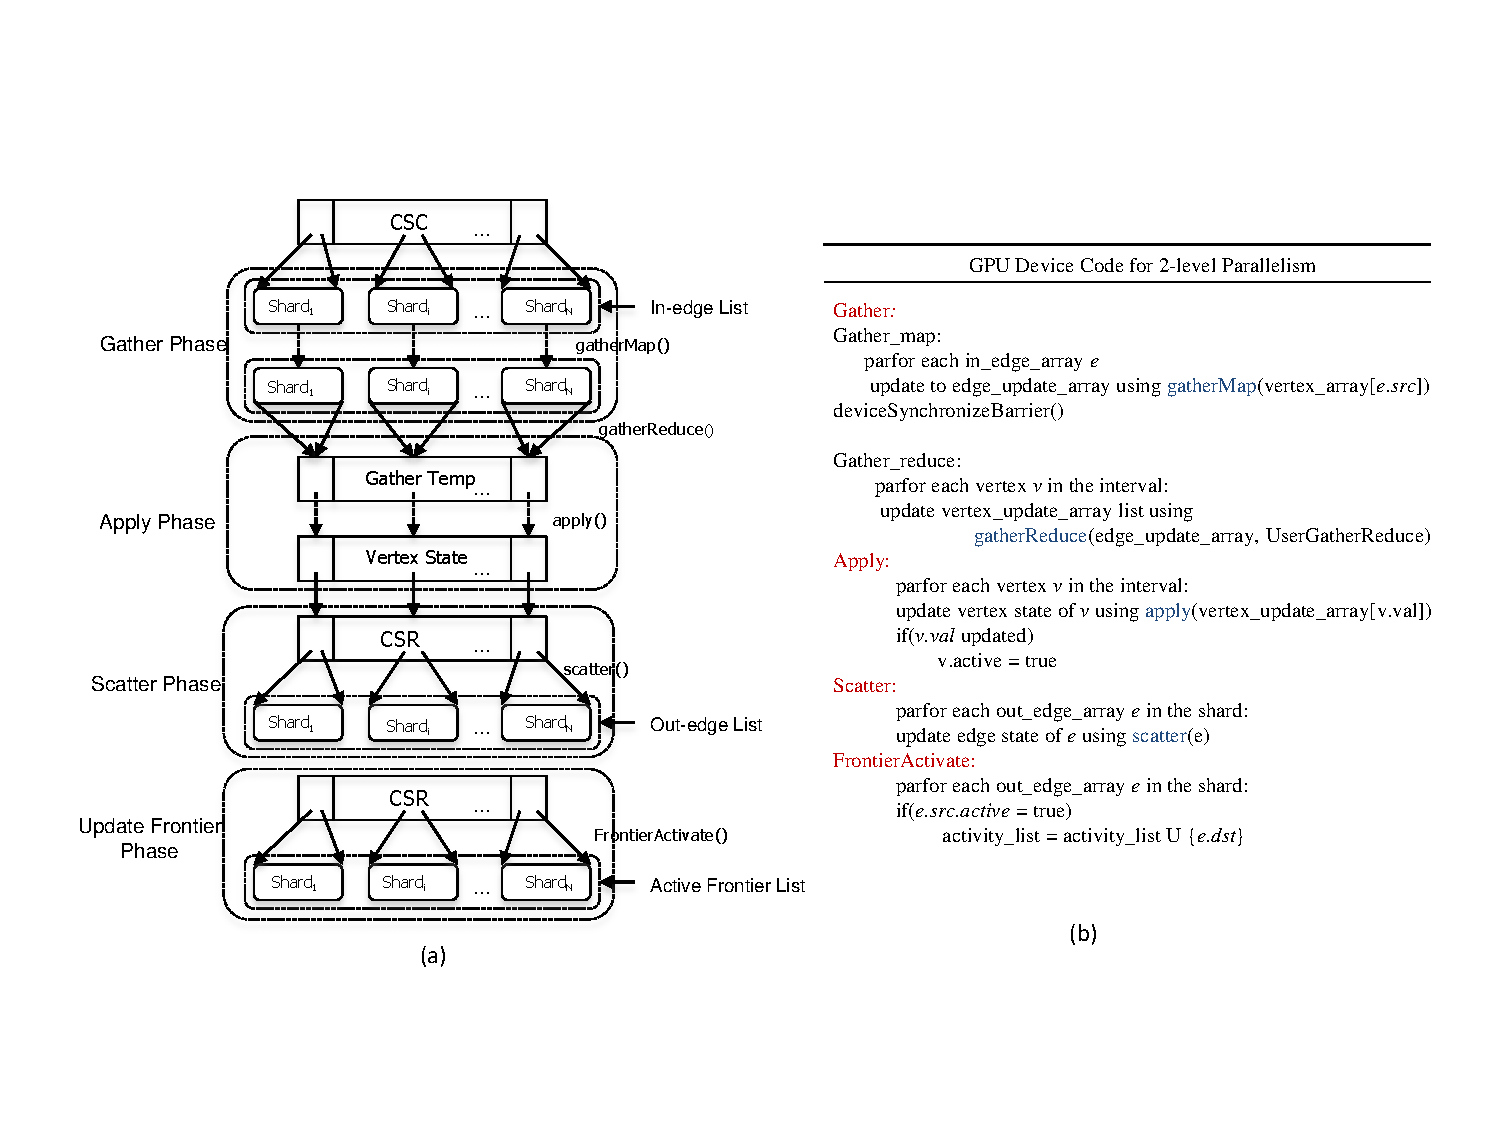
\includegraphics[width=\textwidth,height=\textheight,keepaspectratio]{figures/5phases_1.pdf}
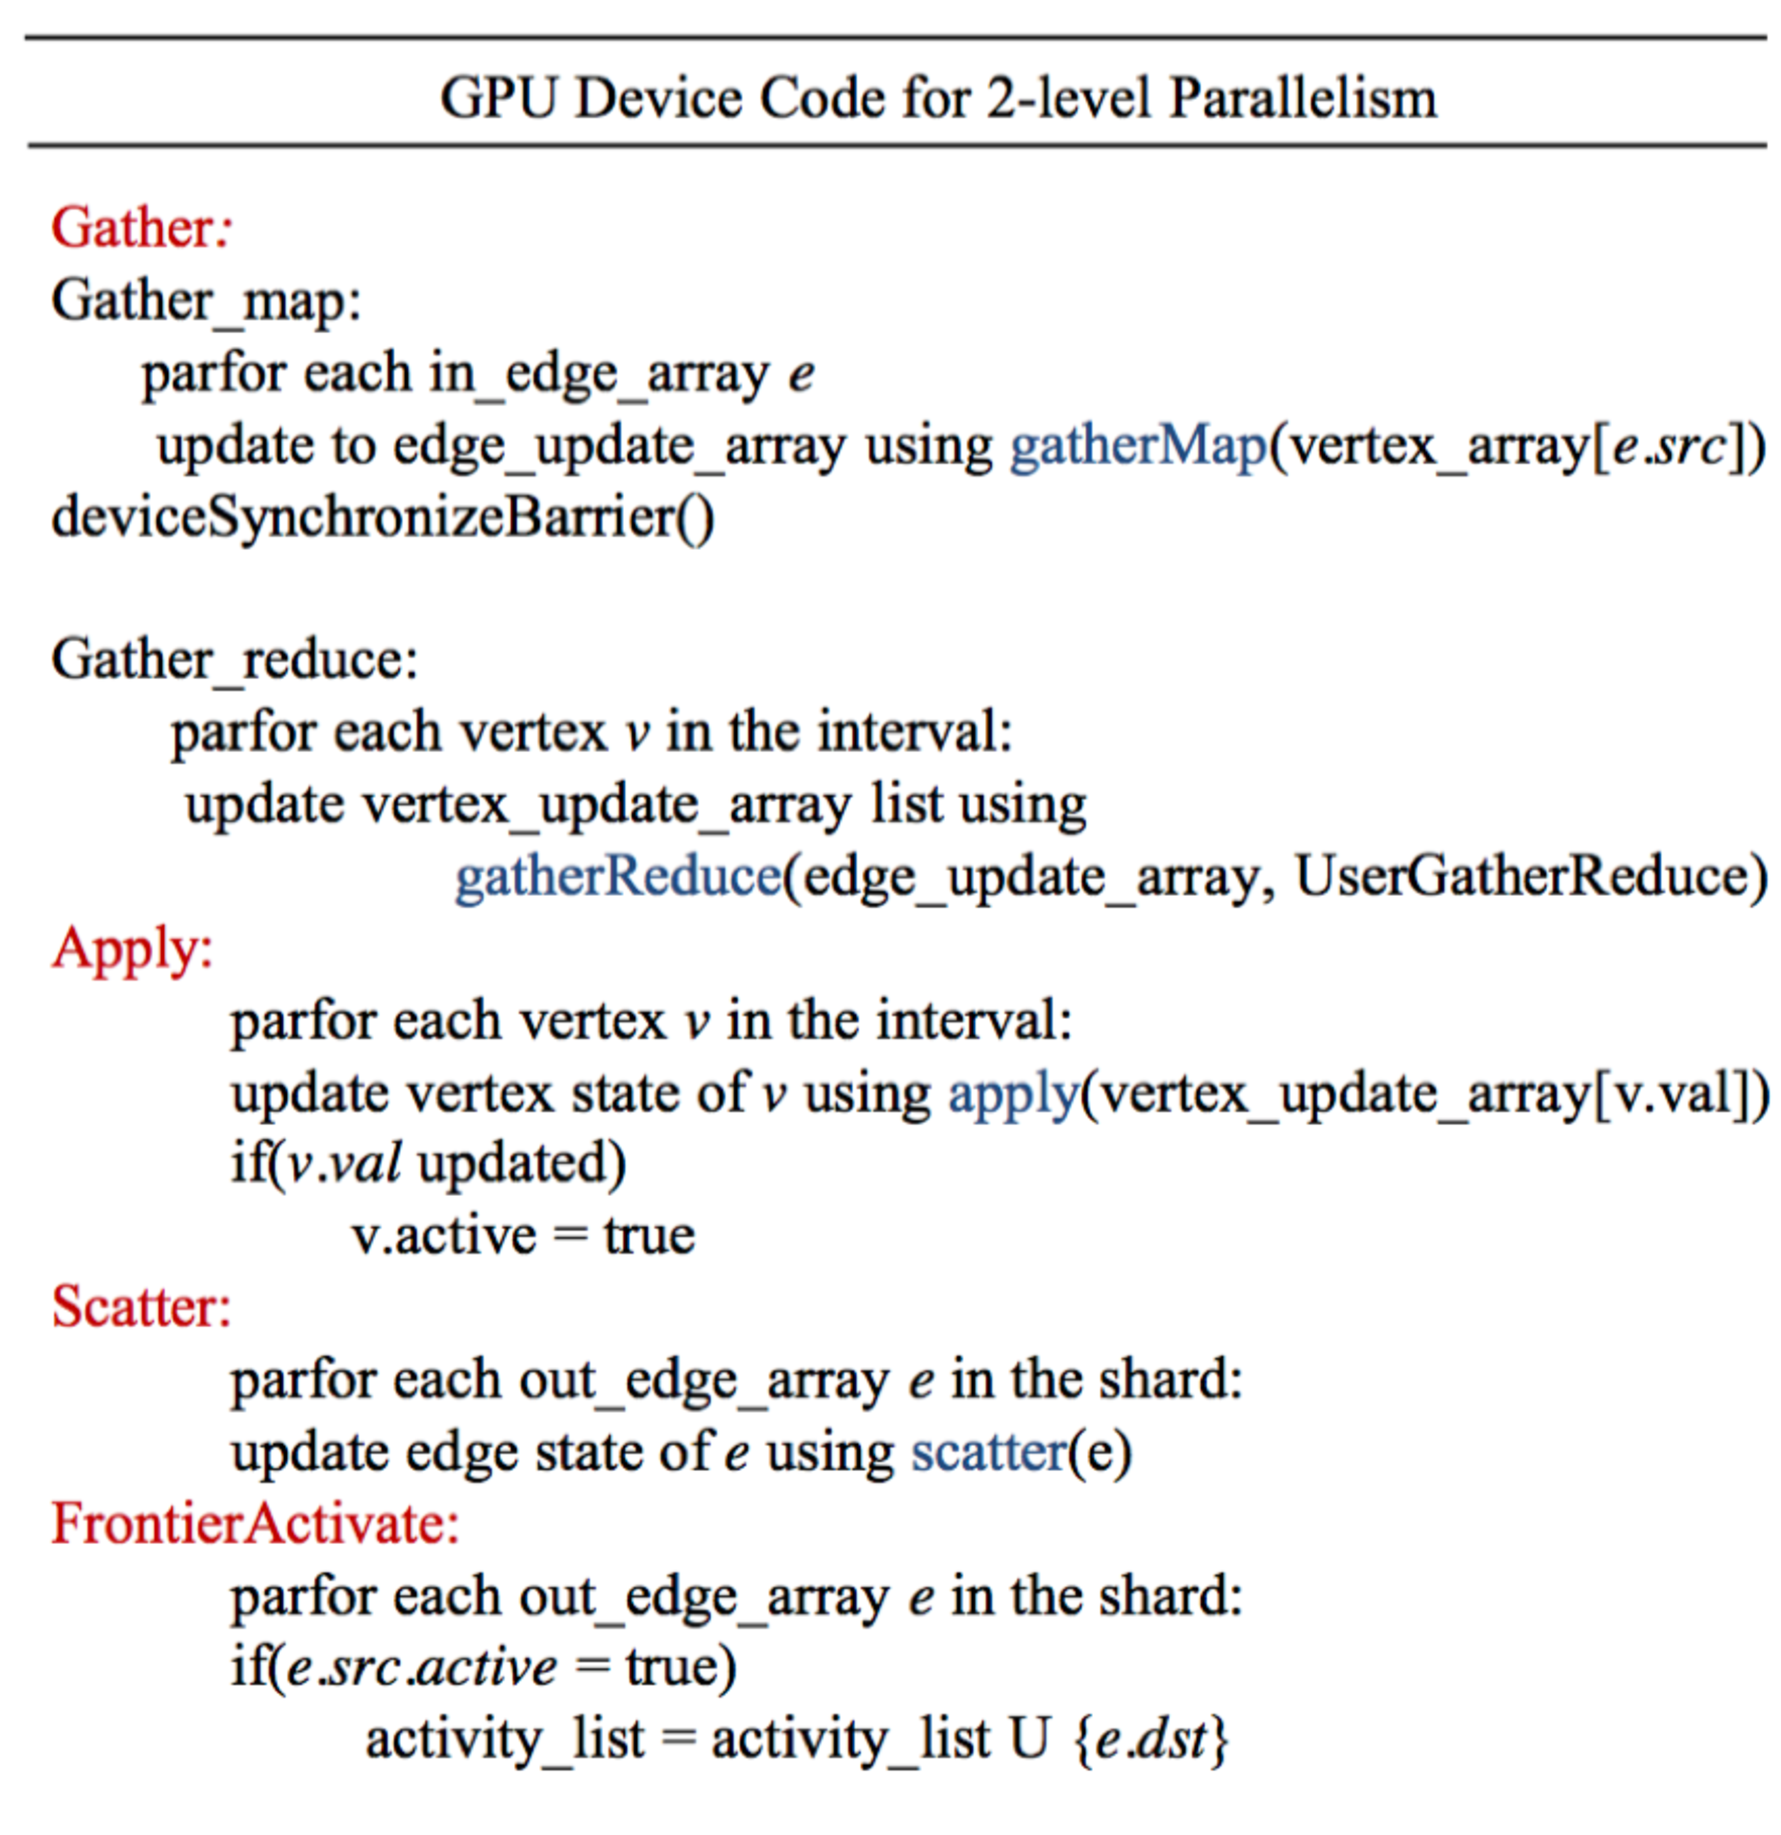
\includegraphics[width=0.85\textwidth,height=\textheight,keepaspectratio]{figures/device_code.pdf}
\caption{GPU device pseudo code for exploiting two-level parallelism in different phases. }
\label{fig:pseudo}
%\vspace{-1\baselineskip}
\end{figure}



Recall the shard data structure illustrated in Figure \ref{fig:shard}, where edge\_update\_array and vertex\_update\_array are 
the update lists of the vertices and their in-edges, respectively, in the corresponding interval (or shard). 
They store the updates from the $Gather$ and $Scatter$ phases of the programming model, shown in Figure \ref{fig:5phases}. 
With these data structures at the very top level, GraphReduce implements a variation of the GAS programming model \cite{pregel,powergraph,graphlab}, shown 
in Figure \ref{fig:pseudo}. It includes the following five phases, where every iteration is over all shards instead of
all edges:


%\vspace{-0.5\baselineskip}
\begin{itemize}
  \item    $gatherMap$: this function fetches all the updates and messages along the in-edges, getting each edge the state of the source vertex and updating that in the edge\_update\_array or GatherTemp data structure. 
 %\vspace{-0.5\baselineskip}
  \item $gatherReduce$: reduces all the collected updates for each vertex with the reduction function defined by programmers. 
 %\vspace{-0.5\baselineskip}
  \item  $apply$: applies reduced updates to each vertex to obtain new states for the vertices. 
%\vspace{-0.5\baselineskip}
 \item  $scatter$: distributes the updated states of the vertices along the out-edges, i.e., update the edge states of the out-edges of the vertices in each shard. In this phase, only the edge states are updated (if the algorithm allows mutable edge states). 
%\vspace{-0.5\baselineskip}
\item FrontierActivate: marks the set of edges and vertices that would be active in the next iteration. \textit{This phase is not user-defined but auto-generated by the GR framework}.
%\vspace{-0.5\baselineskip}
\end{itemize}




For each phase in Figure \ref{fig:pseudo}, GraphReduce requires memcpy-in and memcpy-out operations so as to process all shards
of the entire graph. The next phase will not start until the previous phase has been completed (following the model of 
Bulk Synchronous Parallelism). This can be optimized through dynamic phase fusion and elimination through the \textit{Phase Fusion Engine} inside the Compute Engine, discussed in Section 3.4.3. 

Parallelism in different phases exists at two levels. First, operations are run concurrently within each shard in a given phase.
Second, in a given phase, computation across different shards can also be executed concurrently (i.e., multiple shards residing 
in GPU memory at the same time), because there are no data dependencies between shards in the same phase. 
The device code in Figure \ref{fig:pseudo} shows how GraphReduce exploits this two-level parallelism. This also motivates 
the use of a hybrid programming model explained in Section 3.2.1, as we use an edge-centric implementation for gatherMap, 
scatter, and FrontierActivate phases, but use a vertex-centric implementation for the gatherReduce and apply phases.

Note that the \textit{Function Pointer Table} inside the Compute Engine can take user-defined load-balancing strategies as plug-ins. In the current version of GraphReduce, we apply \textit{CTA (Cooperative Thread Array) load balancing} from the Modern GPU library \cite{moderngpu}. Scan operations and mergesorts are also implemented using the Modern GPU library.


Figure \ref{fig:big_new} also shows the data structures and modules embedded in \textbf{3.} 

(1) {\bf Function Pointer Table}: With adaptivity in mind, Function Pointer Table can take user-defined optimizations as plug-ins. In the current GraphReduce, we apply \textit{CTA load balancing}~\cite{moderngpu}. Scan operations and mergesorts are implemented using modern GPU library \cite{moderngpu}.

(2) {\bf Frontier Manager}: It maintains a list of vertices whose states have changed in the current iteration, and then determines the set of vertices which will be active in the next iteration (details in Section 3.4.2).  

(3) {\bf Phase Fusion and Elimination}:  analyzes if the phases can be merged or even eliminated and based on the phase fusion decision from the Data Movement Engine via phase Synchronization module (details in Section 3.4.3).

(4) {\bf Compute Dispatcher}: It is the core of the Compute Engine which offloads computation operations onto GPU. It is also responsible for using the activity information of the edges to load balance the threads.

(5) {\bf Phase Synchronizer}: It is the control unit manages computation phases and iterations. It is responsible for the synchronization between the compute and data modules, and updating the decision table for fusion/phase elimination optimizations.


\begin{figure}[!t]
\centering
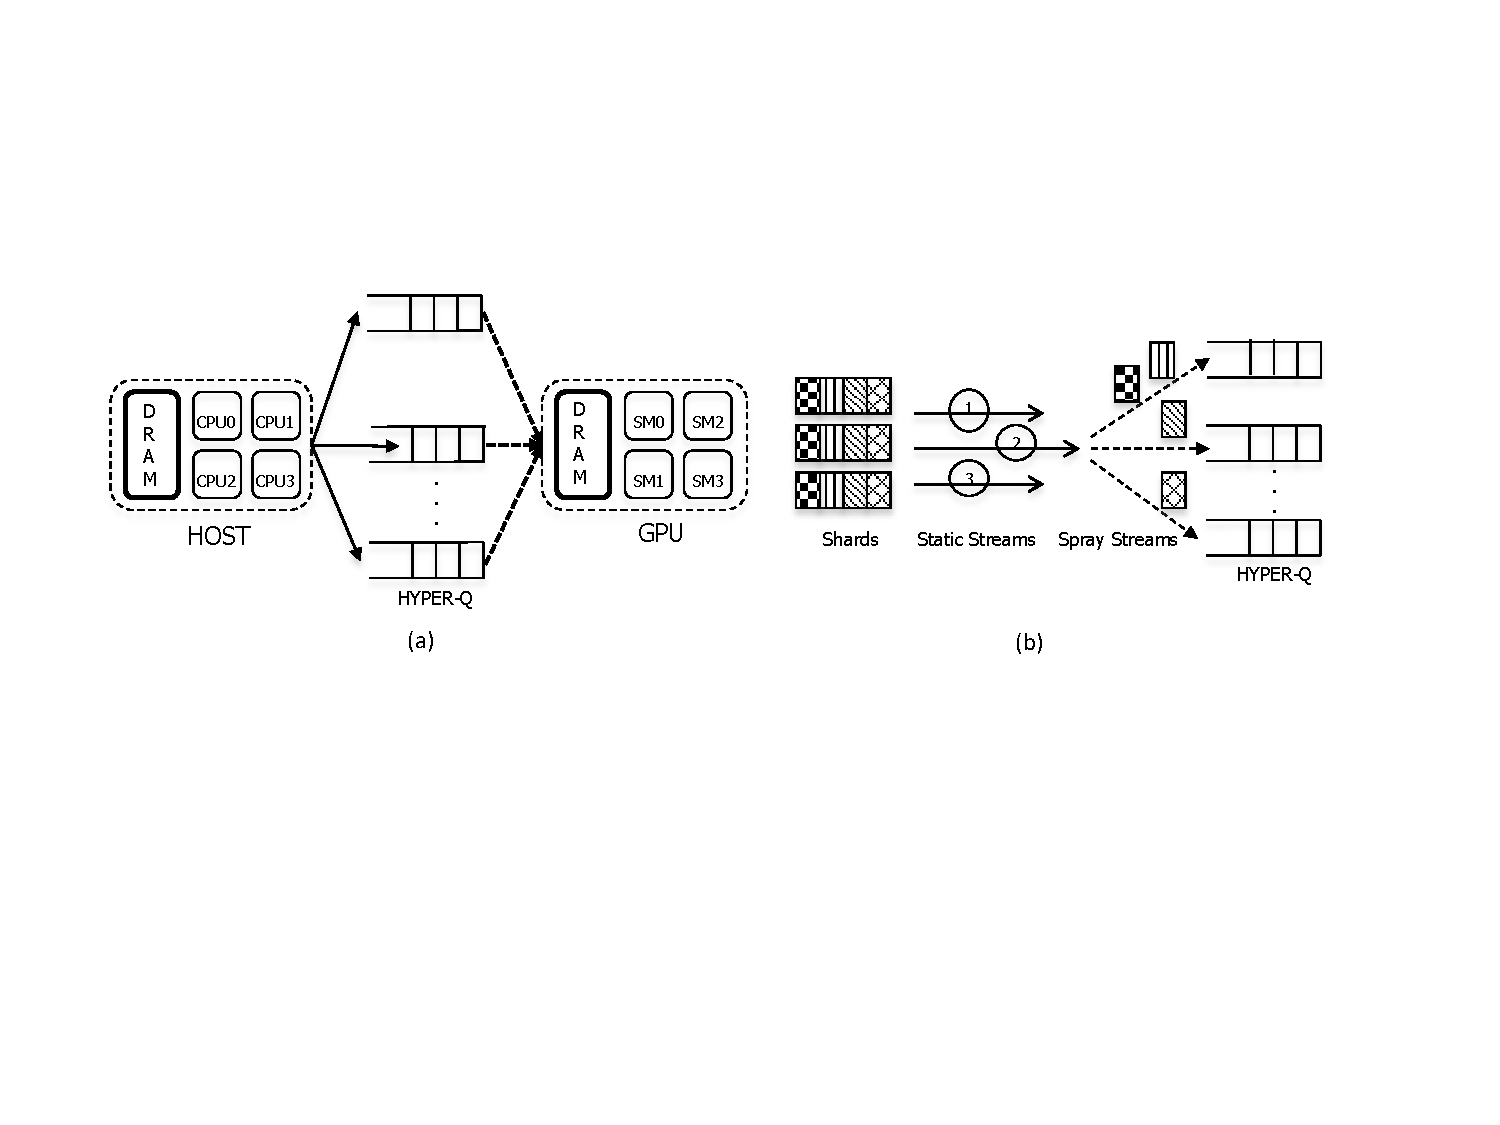
\includegraphics[width=\textwidth,height=\textheight,keepaspectratio]{figures/hyperq.pdf}
\caption{(a) Data Movement from host to GPU in GraphReduce through Hyper-Q. (b) Illustration of Spray Streams for better throughput.}
\label{fig:hyperq}
%\vspace{-1\baselineskip}
\end{figure}
%Optimization

\section{Optimizations}
\label{Optimization}



%\vspace{-0.5\baselineskip}

\subsection{Asynchronous Execution and the Spray Operation}
\label{opt1}


GraphReduce asynchronously performs computation and communication. Specifically, it leverages CUDA Streams, 
double buffering, and hardware support like Hyper-Qs provided by architectures like NVIDIA's Kepler, 
to enable data streaming and computation in parallel. As shown in Figure \ref{fig:big_new}, the \textit{Static Stream Creator} of the 
Data Movement Engine spawns separate CUDA Streams to launch multiple kernels and to transfer data asynchronously, 
overlapping memory copies within and across phases of computation. Novelty in GraphReduce is its use of separate 
CUDA Streams for {\bf deep copy operations}, in order to take advantage of the large number of hardware queues offered 
by modern GPU architectures. This is motivated by the fact that a shard in GraphReduce is not a single contiguous 
byte-array, but consists of many sub-arrays containing edge, vertex, and frontier data. Each of these sub-arrays 
requires a separate deep copy to move data between GPU and host. GraphReduce exploits this fact, as shown in 
Figure \ref{fig:hyperq}(b), by not moving the entire shard in one copy performed by a single CUDA stream, 
but instead, the \textit{Spray Stream Creator} in \textbf{2 }dynamically spawns multiple CUDA Streams 
to move these sub-arrays to the GPU. The outcome is concurrent use of the GPU's many hardware queues, which
consequently improves overall throughput.


%\vspace{-0.5\baselineskip}

\subsection{Dynamic Frontier Management}
\label{opt2}

As discussed in Section 3.1.2, with irregularity in graph processing, in every computation iteration, the frontier size 
is not constant, varying with graph algorithms and datasets. For instance, as shown in Figure \ref{fig:frontier}(c), 
for dataset Cage-15 processed through BFS, only one vertex is active for the first iteration. Inactive vertices or 
edges in each iteration can result in significant performance degradation due to GPU thread idling. 
To address this problem, we integrate the \textit{Frontier Manager module} into the Computation Engine to maintain the list of active vertices whose states have changed in the current iteration and uses it to determine the set of vertices in one hop neighborhood that will be active in the next iteration (based on out-edges information in a shard). GraphReduce then uses this frontier information of the \textit{next} iteration to avoid unnecessary memcpys and kernel launching. It also uses the active vertex information of the \textit{current} iteration for CTA load balancing to avoid GPU core idling.

 


%\vspace{-0.5\baselineskip}

\subsection{Dynamic Phase Fusion/Elimination}
\label{opt3}


A graph algorithm implemented with GraphReduce need not implement user-defined functions for all three GAS phases. 
For example, BFS need not implement the Scatter phase. In response, when a phase is elided by the user, 
GraphReduce eliminates the repeated and unnecessary movement of shards into GPU memory, before and after that phase, 
in each iteration. This is termed phase elimination. For instance, if the graph algorithm does not have a defined 
gather function, GraphReduce will avoid bringing in the entire shard (in-edges+out-edges), only moving the out-edges 
to the GPU memory (because in-edges are used only in the Gather phase). Out-edges are moved regardless, because
the FrontierActivate phase operates even when there is no scatter phase defined. The resulting dynamic phase elimination 
reduces unnecessary kernel launching and data movement. 

In certain scenarios, merging two or more GAS phases is possible, again to avoid unnecessary extra data movement. 
For example, if a graph algorithm only defines Apply and FrontierActivate phases, GraphReduce will automatically merge 
these two phases, thus avoiding the \textit{memcopy} operations that would have been required for executing the two phases 
separately. We term this action dynamic phase fusion. An example of a graph algorithm for which this method is used
is again BFS. It only requires users to define the apply phase, in which the BFS tree depth for every vertex is marked 
to be the iteration number. GraphReduce will automatically merge the Apply and FrontierActivate phases for BFS. Note that Dynamic Fusion/Elimination functionalities are enabled
through the \textit{Phase Fusion Engine} inside the Compute Engine.




Other minor optimizations introduced in the GR frame- work include: 1) if the shards fit in the memory then there is no need to write back the edge state to the host. Subsequent phases and iterations reuse the shard in its computation. Similarly, if the vertex array fits in the memory then no need to write it back to the host after each iteration. 2) avoid unnecessary write back of temporary states like the gatherTemp to host which will be overwritten in the next iteration anyway. To implement this GR uses the read/write attribute information from the Buffer-list. 

%Experiment Section
\section{Experimental Evaluation }
\label{experiment}

\subsection{Experimental Setup}

\textbf{Evaluation Platform:} GraphReduce is evaluated on a typical heterogeneous HPC node equipped with 16-core Intel Xeon E5-2670 processors running at 2.6 GHz with 32 GB of DDR3 RAM, and one attached NVIDIA Tesla K20c GPU with 13 SMX multiprocessors and 4.8 GB GDDR5 RAM. The Kepler GPU is enabled with CUDA 6.5 runtime and the version 340.29 driver, while the host CPU side is running Fedora version 20 with kernel v.3.11.10-301 x86. All the runs are compiled with the highest optimization level flag.  

% Please add the following required packages to your document preamble:
% \usepackage{graphicx}


\textbf{Graph Dataset.} Shown in Table \ref{datasets}, we evaluate the performance and efficiency of GraphReduce using two types of graph inputs: 
small size graphs that will fit into GPU memory (named In-memory graphs) and large graphs that do not fit (named Out-of-memory graphs). 
Here, we define the size of a graph as the amount of memory required to store the edges, vertices, and edge/vertex data states in terms of 
the user-defined datatypes and a few of the temporary buffers. All experiments use datatype \textit{float}. Note that the size of a graph 
can expand after loading it to in-memory buffers, because the size of the datatypes for edge and vertex states is in general larger than 
their representations in the raw graph format (e.g., \textit{char}). 

In-memory graphs are used to evaluate the effectiveness of GraphReduce's in-memory optimizations against other state-of-the-art in-memory 
approaches (e.g., MapGraph and CuSha), while Out-of-memory graphs are used to evaluate it against frameworks that can process large graph 
sets (e.g., GraphChi and X-Stream). 

The ten real-world graphs listed in Table \ref{datasets} are publicly available and cover a wide range of sparsity and sizes. 
For example, \textit{orkut} is an undirected social network, in which vertices and edges represent the friendship between users. 
\textit{uk-2002} is a large crawl of the \textit{.uk} domains, in which vertices are the pages and edges are the links. 
\textit{nlpkkt160} is from the 3D PDE-constrained optimization problem with vertices as state variables and edges as control variables. 

\textbf{Evaluated Algorithms.} Four widely used algorithms are evaluated, including Breadth First search (BFS), Page Rank (PR), 
Single-Source Shortest Paths (SSSP), and Connected Components (CC). Algorithms requiring undirected graphs as inputs, e.g., 
connected components, are stored as pairs of directed edges.


%\vspace{-0.5\baselineskip}


\subsection{Evaluation and Analysis}
\label{6.1}





% Please add the following required packages to your document preamble:
% \usepackage{multirow}
\begin{table}[h]%\scriptsize
\centering
\begin{tabular}{|c|c|c|c|c|c|}
\hline
Graph &  & BFS & SSSP & Pagerank & CC \\ \hline
\multirow{3}{*}{kron-logn21} & GraphChi & 365 & 442 & 328 & 236 \\ \cline{2-6} 
 & Xstream & 95 & 97 & 98 & 97 \\ \cline{2-6} 
 & GR & 4 & 7 & 93 & 9 \\ \hline
\multirow{3}{*}{nlpkkt160} & GraphChi & 503 & 510 & 447 & 1560 \\ \cline{2-6} 
 & Xstream & 128 & 136 & 144 & 133 \\ \cline{2-6} 
 & GR & 60 & 92 & 140 & 183 \\ \hline
\multirow{3}{*}{uk-2002} & GraphChi & 1100 & 1283 & 1091 & 1073 \\ \cline{2-6} 
 & Xstream & 330 & 374 & 335 & 348 \\ \cline{2-6} 
 & GR & 49 & 80 & 153 & 162 \\ \hline
\multirow{3}{*}{orkut} & GraphChi & 311 & 320 & 285 & 268 \\ \cline{2-6} 
 & Xstream & 124 & 131 & 127 & 127 \\ \cline{2-6} 
 & GR & 6 & 10 & 84 & 16 \\ \hline
\multirow{3}{*}{cage15} & GraphChi & 262 & 265 & 240 & 389 \\ \cline{2-6} 
 & Xstream & 114 & 119 & 115 & 143 \\ \cline{2-6} 
 & GR & 18 & 25 & 19 & 41 \\ \hline
\end{tabular}
\caption{Execution times of out-of-memory graph processing frameworks on different algorithms and graph inputs. Reported times are wall time and in {\bf seconds}.}
\label{bigdata}
%\vspace{-1\baselineskip}
\end{table}


% Please add the following required packages to your document preamble:
% \usepackage{multirow}
\begin{table}[h]%\scriptsize
\centering
\begin{tabular}{|c|c|c|c|c|c|}
\hline
Graph &  & BFS & SSSP & Pagerank & CC \\ \hline
\multirow{3}{*}{ak2010} & MG & 7.94 & 79.01 & 23.86 & 19.03 \\ \cline{2-6} 
 & CuSha & 7.75 & 31.99 & 12.08 & 10.16 \\ \cline{2-6} 
 & GR & 9.26 & 3.81 & 14.61 & 17.78 \\ \hline
\multirow{3}{*}{coAuthorsDBLP} & MG & 5.28 & 8.75 & 68.92 & 30.26 \\ \cline{2-6} 
 & CuSha & 11.55 & 12.75 & 79.84 & 13.99 \\ \cline{2-6} 
 & GR & 5.31 & 5.42 & 53.14 & 16.43 \\ \hline
\multirow{3}{*}{kron-logn20} & MG & 51.81 & 139.43 & 6789 & 308.91 \\ \cline{2-6} 
 & CuSha & 119.82 & 269.88 & 1852 & 138.7 \\ \cline{2-6} 
 & GR & 27.88 & 28.34 & 4365 & 266.86 \\ \hline
\multirow{3}{*}{webbase-1M} & MG & 8.71 & 13.56 & 72.86 & 50.97 \\ \cline{2-6} 
 & CuSha & 13.52 & 12.65 & 270.83 & 317.41 \\ \cline{2-6} 
 & GR & 1.4 & 6.07 & 57.76 & 37.45 \\ \hline
\multirow{3}{*}{belgium\_osm} & MG & 195.79 & 261.32 & 102.64 & 2219 \\ \cline{2-6} 
 & CuSha & 791.3 & 897.03 & 45.8 & 920.7 \\ \cline{2-6} 
 & GR & 279.8 & 281.39 & 71.33 & 40.63 \\ \hline
\end{tabular}
\caption{Performance results of in-memory (small) graph processing frameworks on different algorithms and graph inputs. Reported times are in { milliseconds}. {MG stands for MapGraph.}}
\label{smalldata}
%\vspace{-0.5\baselineskip}
\end{table}


\begin{figure}[!t]
\centering
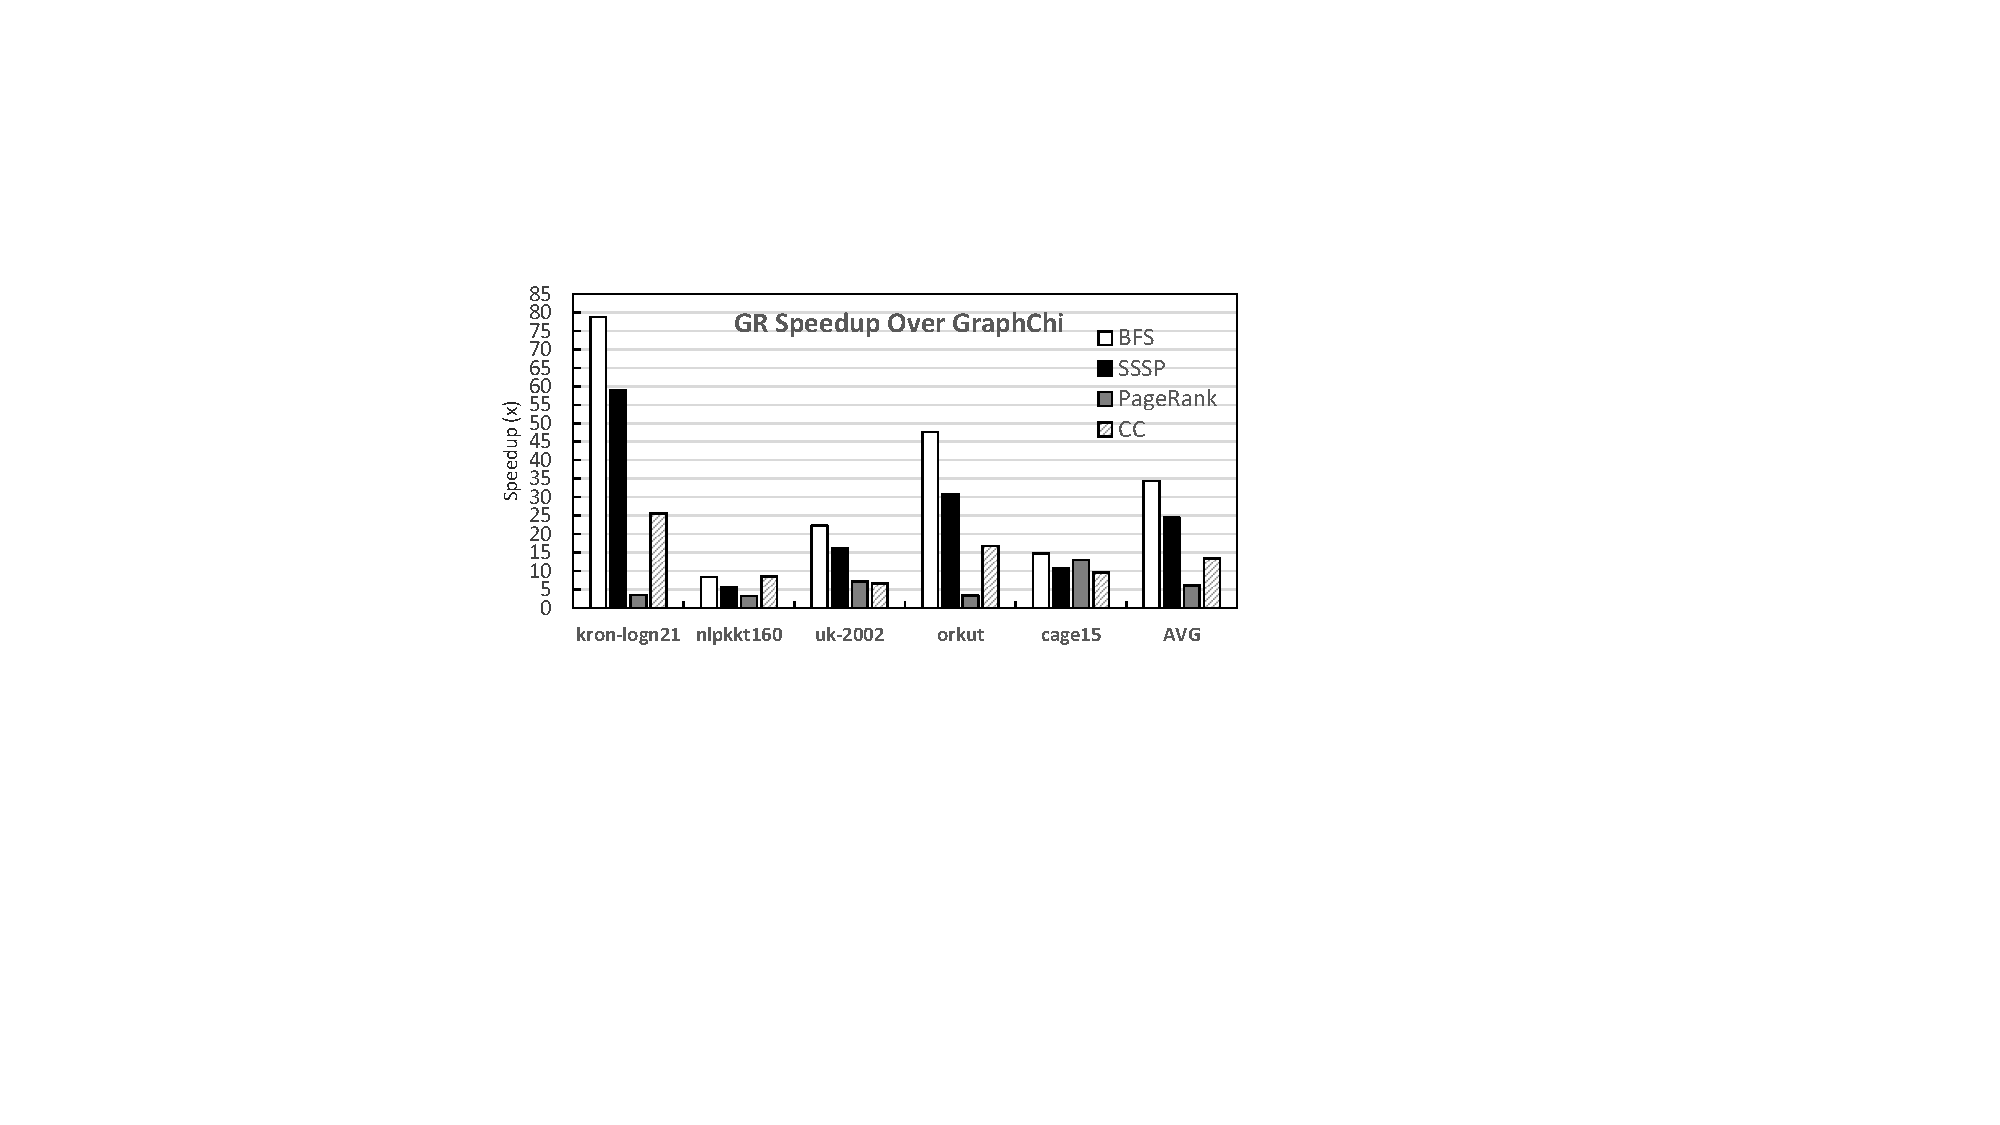
\includegraphics[width=0.75\textwidth,height=0.75\textheight,keepaspectratio]{figures/speedup1.pdf}
\caption{GR's speedup over GraphChi for various algorithms and out-of-memory graph inputs. }
\label{fig:speedup1}
%\vspace{-0.5\baselineskip}
\end{figure}

\begin{figure}[!t]
\centering
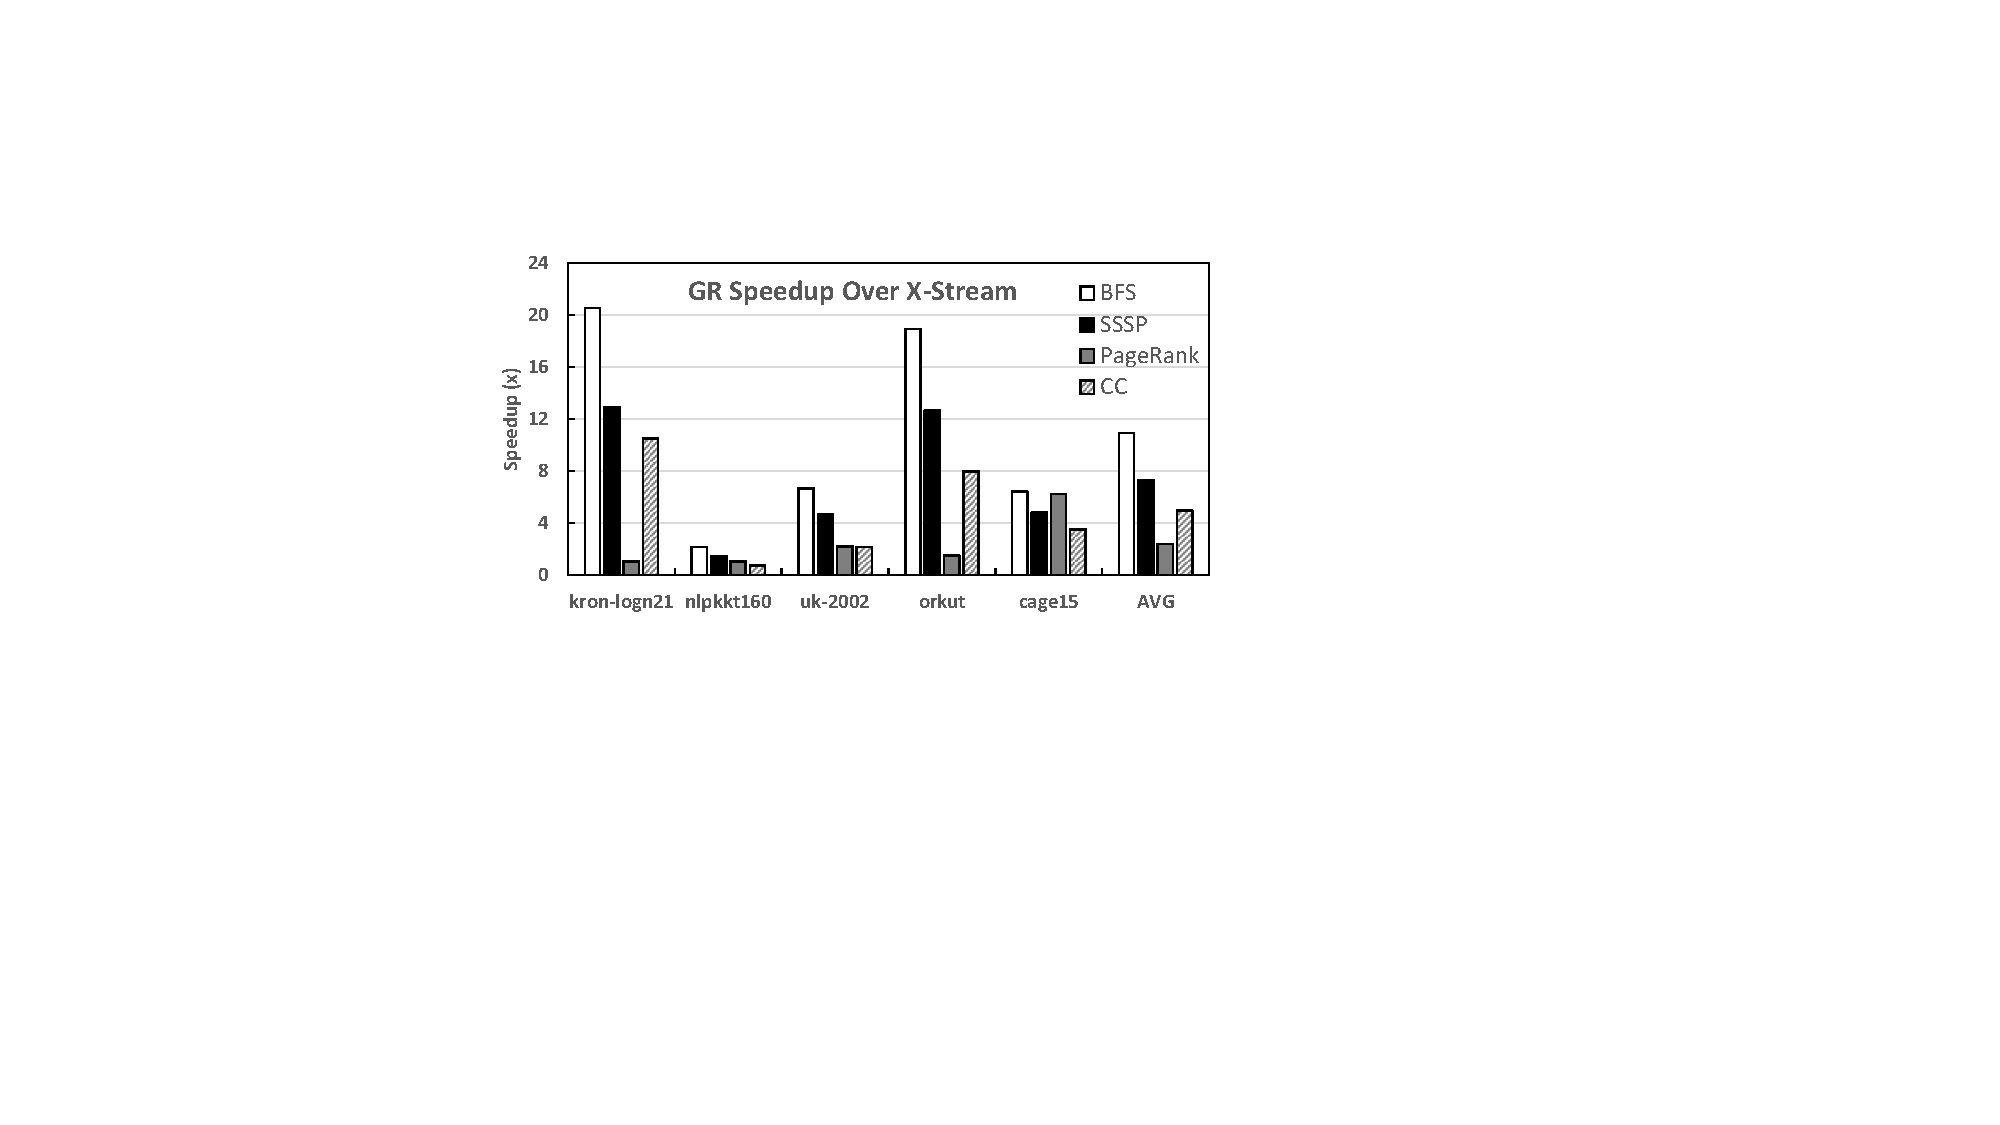
\includegraphics[width=0.75\textwidth,height=0.75\textheight,keepaspectratio]{figures/speedup2.pdf}
\caption{GR's speedup over X-Stream for various algorithms and out-of-memory graph inputs. }
\label{fig:speedup2}
%\vspace{-1\baselineskip}
\end{figure}





\subsubsection{Comparison with Out-of-Memory Frameworks}


Since the state-of-the-art GPU-based graph processing approaches \cite{mapgraph,vertexapi,medusa,cusha} assume that input graphs fit 
in GPU memory, we compare GR's out-of-memory performance with Graphchi \cite{chi} and X-Stream \cite{xstream}, both state-of-the-art, 
out-of-memory, CPU-based frameworks targeting large real-world graphs. For fairness in comparison, the datasets chosen (in-memory sizes 
shown in Table \ref{datasets}) fit in host memory but do not fit into GPU memory. This is to avoid I/O (SSD access) overheads in
systems like GraphChi and X-Stream. GR, however, incurs the unavoidable costs of moving \textit{shards} in and out of GPU memory.


Shown in Table \ref{bigdata}, Figure \ref{fig:speedup1}, and Figure \ref{fig:speedup2}, GR achieves an average speedup of 
{\bf 13.4x and 5x} over GraphChi and X-Stream (running with 16 threads), respectively, despite its need to move data
between GPU and CPU via PCIe; while Graphchi and X-Stream benefit from local (host) memory access. GR achieves some significant speedups, 
e.g., up to 79x over GraphChi and 21x over X-Stream, for kron\_g500-logn21 processed by BFS. These performance improvements are due to
its (i) asynchronous mode and spray operation (leveraging CUDA Streams, Hyper-Qs, and deep memory copy operations); 
(ii) dynamic frontier management, to avoid unnecessary kernel launching and GPU core idling; and (iii) dynamic phase fusion/elimination 
to remove unnecessary data movement. The
hybrid programming model also contributes to the performance improvements over GraphChi and X-Stream, by extracting access pattern-based parallelism opportunities across different phases. GraphChi (vertex-centric) 
and X-Stream (edge-centric), on the other hand, suffer from significant random accesses to either their edge or vertex sets, 
due to their use of a unified model. There is only one case that X-Stream performs slightly better than GR, which is the the nlpkkt160 
input processed by CC. This is due to the fact that GR experiences substantial overheads from the large data movement over PCIe, and these overheads
are not sufficiently compensated by the massive parallelism offered by GPU. GrapChi and X-Stream, in comparison, have all data accessible
locally in the host memory and are therefore, not subject to such overheads. 
%But this issue can be easily addressed when a cc-NUMA type of GPU architecture is put in place in near future \cite{hpca15}. 



%\vspace{-0.5\baselineskip}

\subsubsection{Comparison with GPU In-Memory Frameworks}


The results above establish GR's ability to process large graphs that do not fit into GPU memory, at levels of performance higher than
that seen for CPU-based solutions. In other words, additional costs arising from GPU-host data movement are typically dwarfed by the
performance advantages offered by fast GPUs. At the same time, GR also performs as well as the existing in-GPU-memory solutions 
for smaller graph inputs. Table \ref{smalldata} shows GR's in-memory performance for smaller graphs to be comparable to the state-of-the-art 
in-memory processing frameworks like MapGraph (MG) and CuSha, which apply multi-level fine-tuned optimizations for in-GPU workloads. 
In many cases, GR outperforms MG and CuSha significantly, e.g., kron\_g500-logn20 with SSSP and webbase-1M with BFS. For processing 
these smaller graphs, one major contributing factor for high performance in GR is its use of active vertex information of the same iteration 
for the CTA load balancing. One interesting observation is that not all of the GPU in-memory graph processing approaches work well for every 
graph input and algorithm. This prompts us to (also see Sections 3.3.2 and 3.3.4) to add flexibility to GR's Partition Engine -- the Partition 
Logic Table can be easily modified to incorporate desired user-defined specific optimizations, e.g., to use the partition and graph layout algorithms
employed in CuSha.



%\vspace{-0.5\baselineskip}

\subsubsection{Performance Effects of GraphReduce Optimizations}


\begin{figure}[!t]
\centering
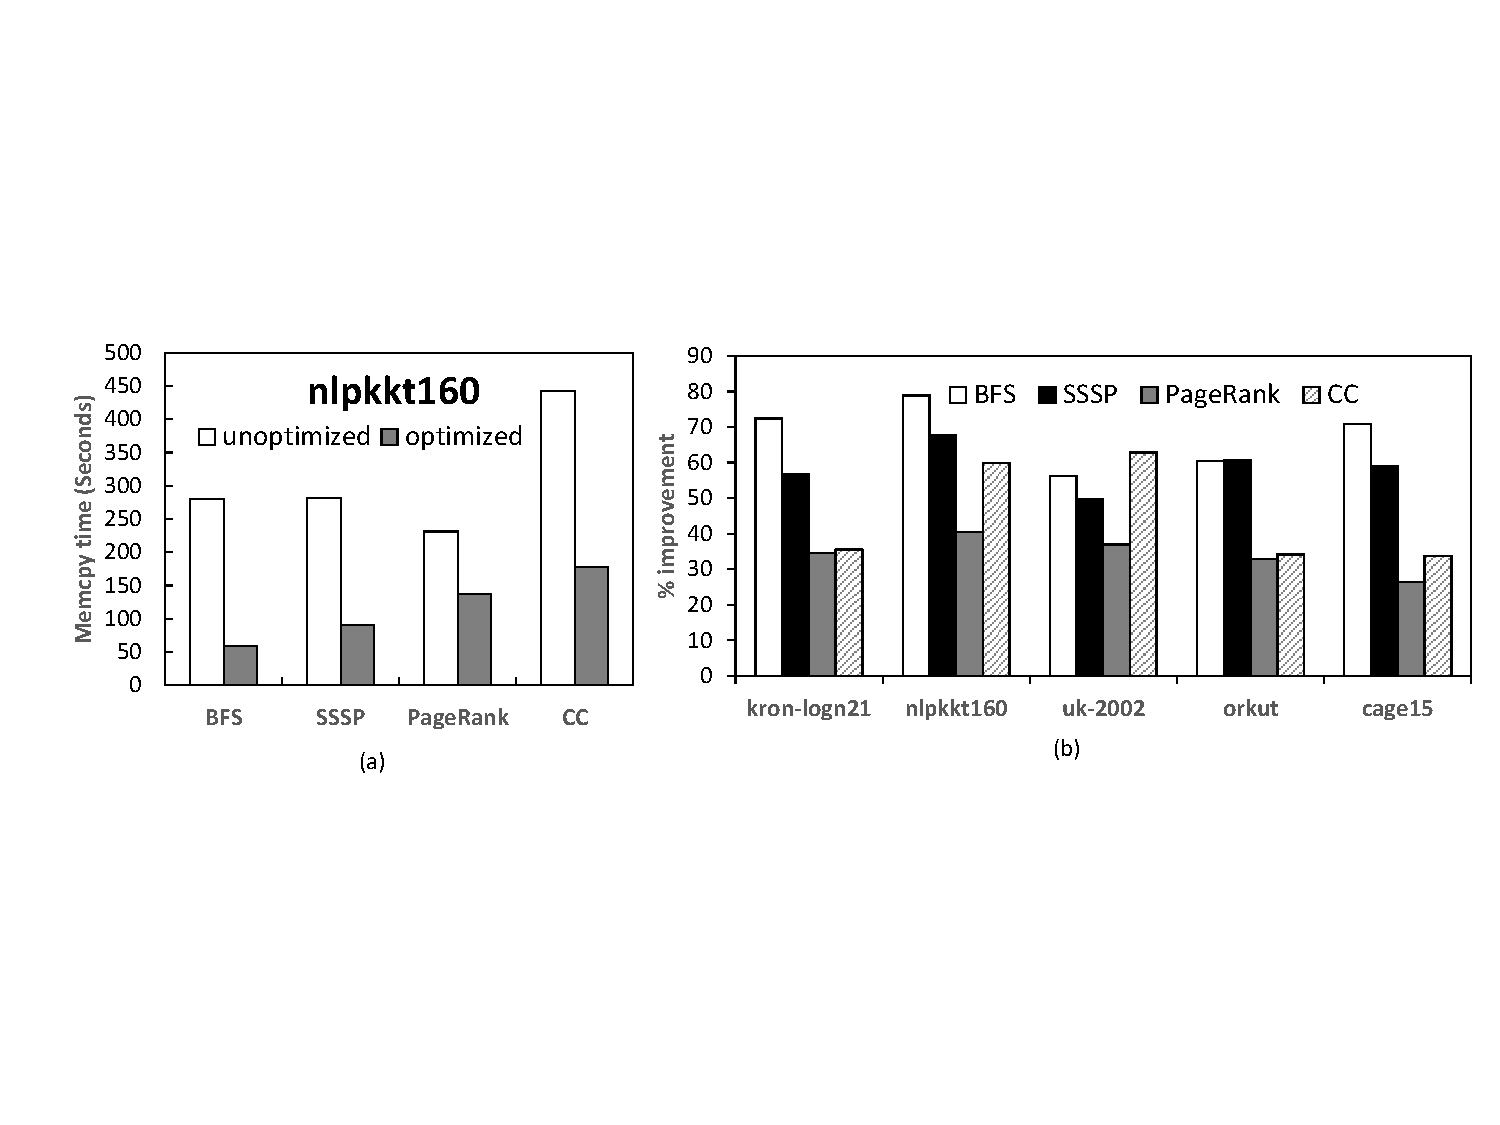
\includegraphics[width=\textwidth,height=\textheight,keepaspectratio]{figures/memcpy.pdf}
\caption{Performance gained from memcpy optimization. (a) Actual memcpy time comparison between optimized and unoptimized GR for nlpktt160. (b) Percentage improvement of memcpy performance from optimized GR against unoptimized GR. }
\label{fig:memcpy}
%\vspace{-0.5\baselineskip}
\end{figure}

\begin{figure}[!t]
\centering
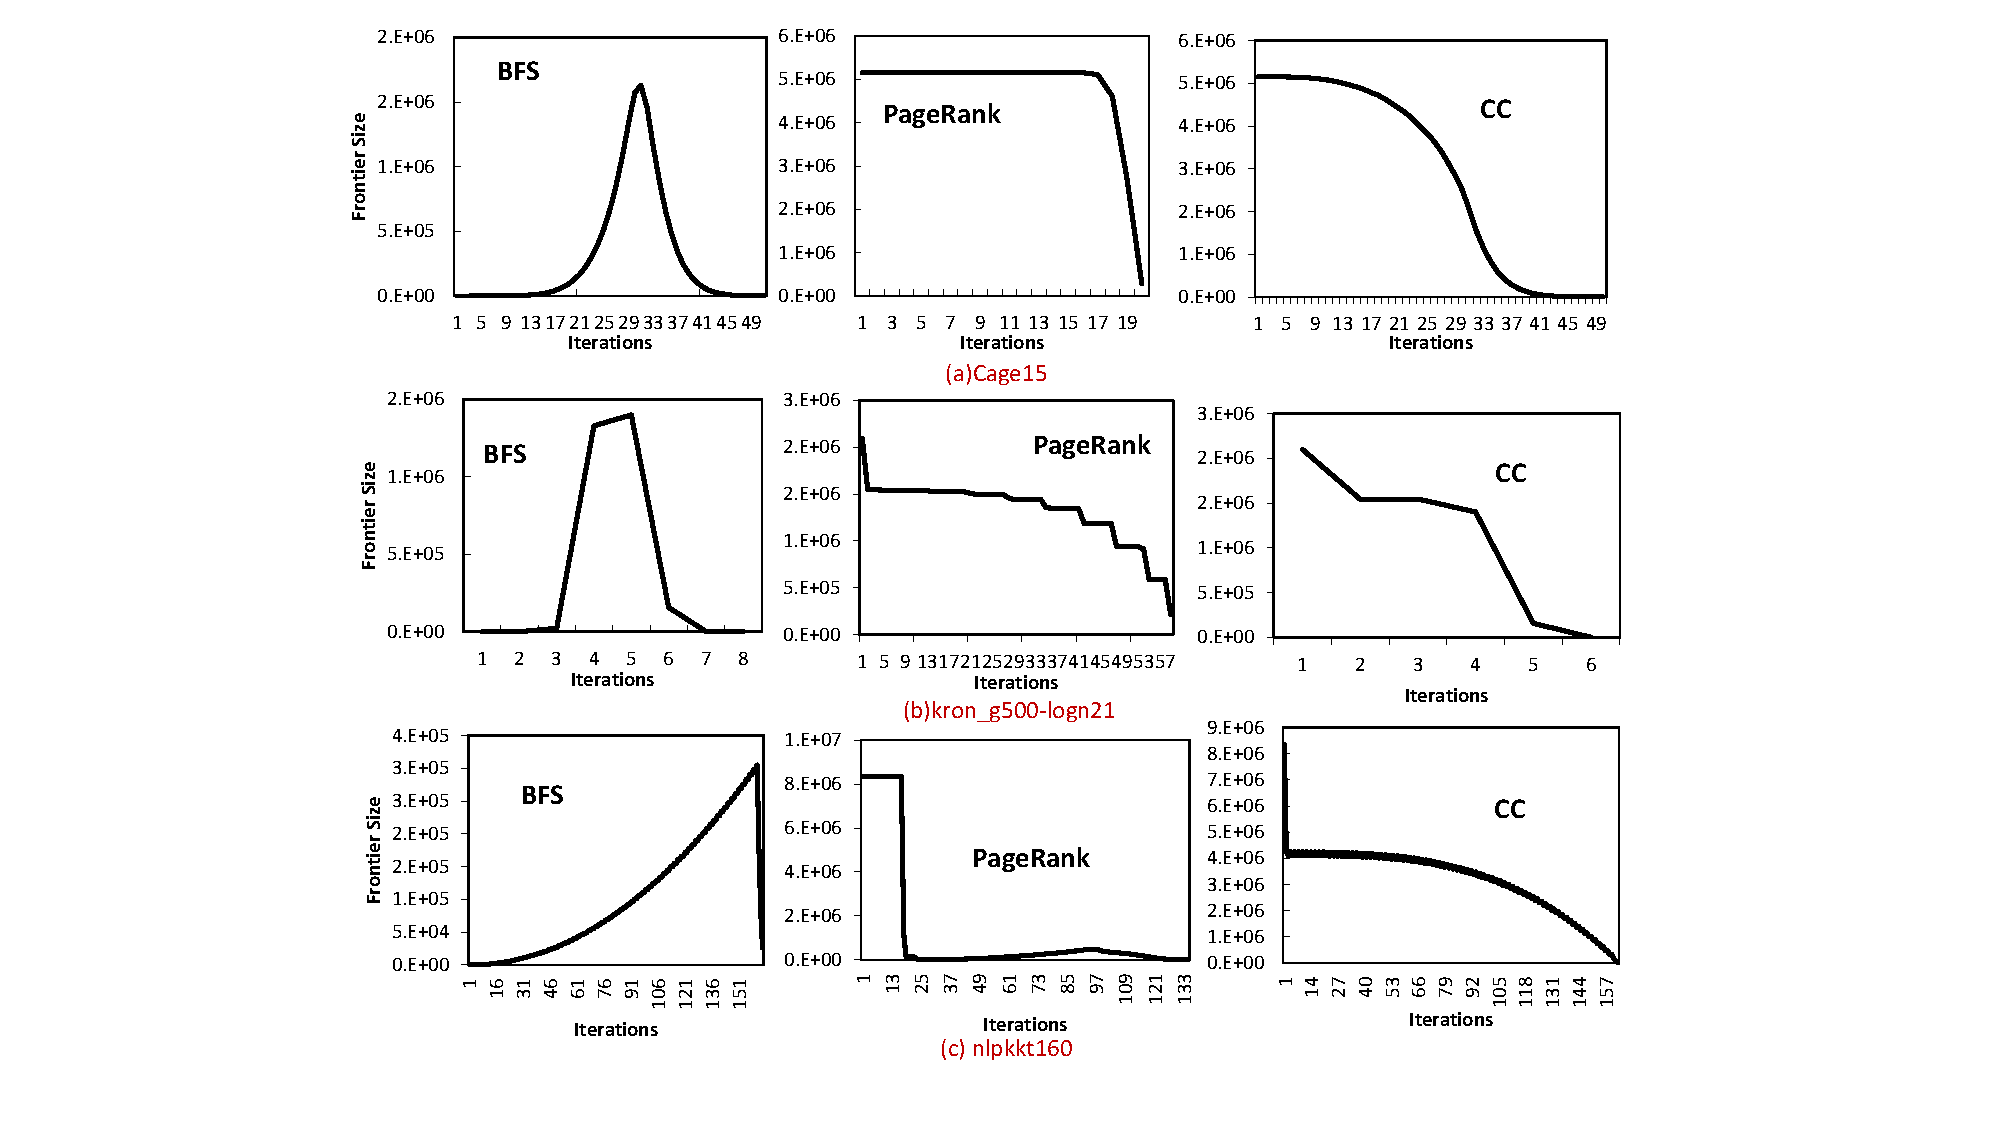
\includegraphics[width=\textwidth,height=\textheight,keepaspectratio]{figures/frontier2.pdf}
\caption{Frontier size changes across iterations shown for several large out-of-memory graphs with three algorithms. 
 }
\label{fig:frontier2}
%\vspace{-0.5\baselineskip}
\end{figure}

\begin{figure}[!t]
\centering
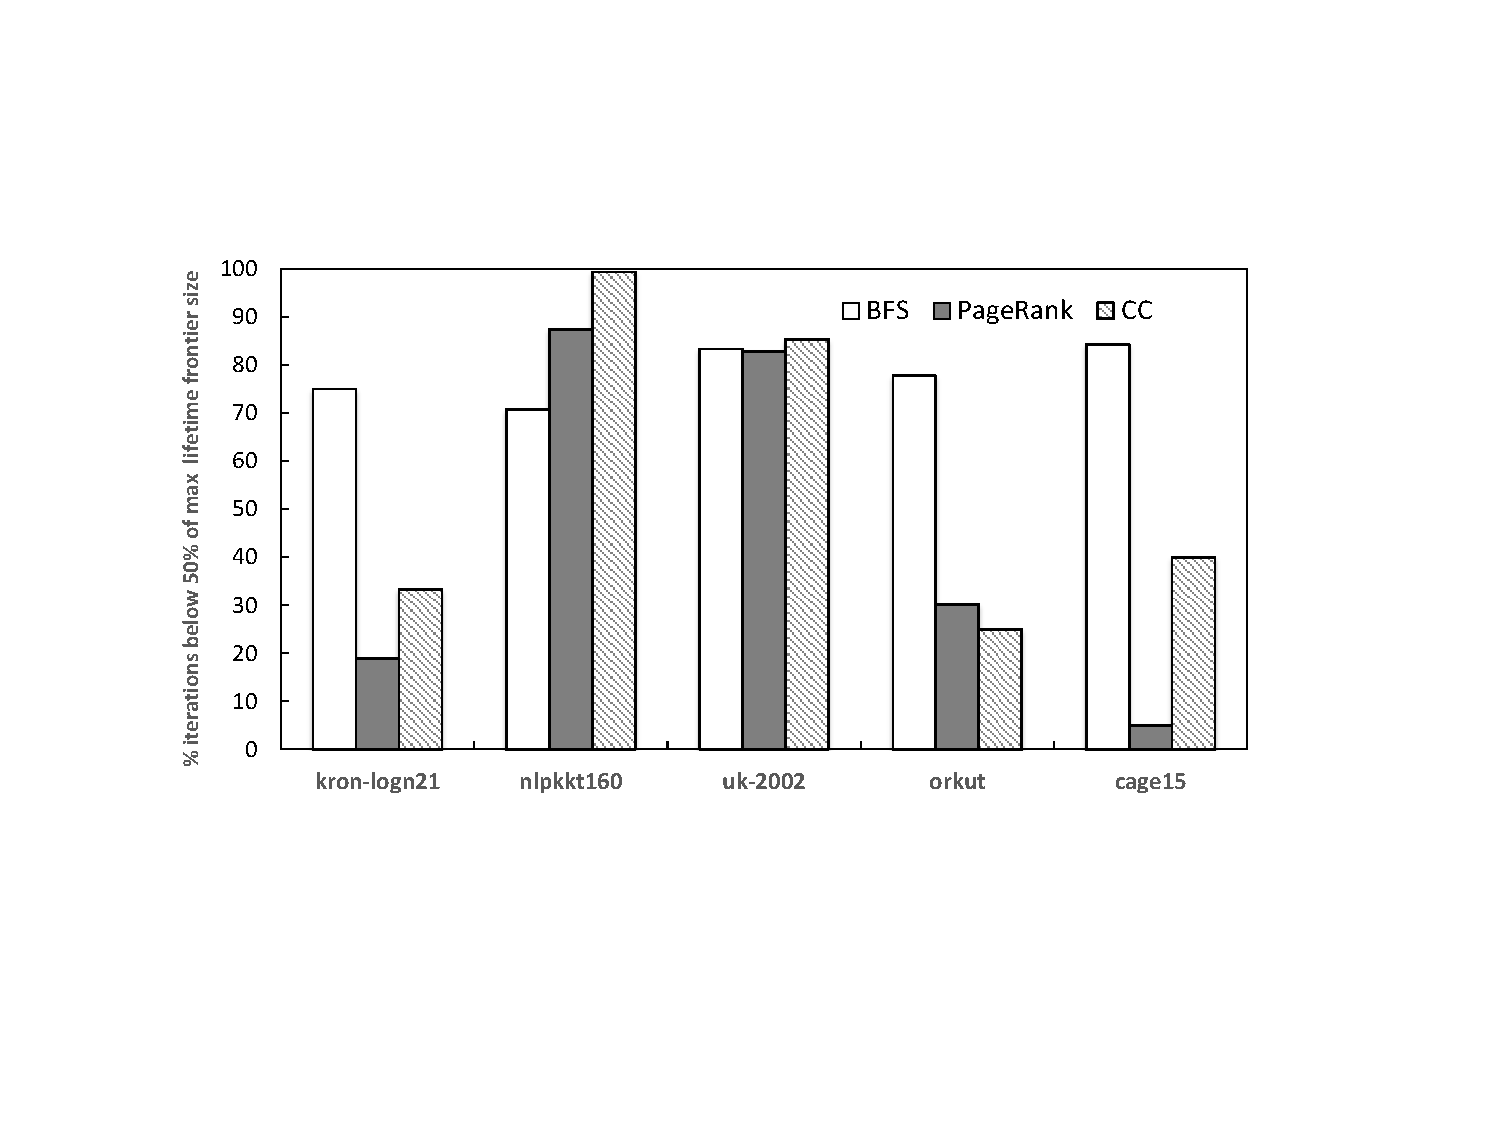
\includegraphics[width=0.75\textwidth,height=0.75\textheight,keepaspectratio]{figures/frontier_exp.pdf}
\caption{For out-of-memory graphs, percentage of iterations that are below 50\% of the max lifetime frontier size.  
 }
\label{fig:frontier_exp}
%\vspace{-1\baselineskip}
\end{figure}


Experimental results show memcpy time to be a dominant factor for performance, occupying on the average above 95\% of the total execution time 
for the five large out-of-memory graph inputs studied above. This makes it the primary target for GR optimizations.
Figure \ref{fig:memcpy} shows the performance improvements gained from the three optimizations discussed in Section 3.4, 
including asynchronous execution/spray operation, dynamic frontier management, and dynamic phase fusion/elimination. 
For example, without these optimizations, Figure \ref{fig:memcpy}(a) shows that the performance of nlpkkt160 suffers significantly from memcpy, 
e.g., up to 443 seconds for the CC with the total execution time only being 451 seconds. With the optimizations, memcpy time drops from 
443 seconds to 178 seconds, improved by 60\%. Figure \ref{fig:memcpy}(b) shows the percentage improvement of memcpy time from 
the optimized GR over the baseline unoptimized scenario, with an average of 51.5\% and up to 78.8 \% across all large datasets and algorithms. 



A simple example shows how dynamic frontier management affects memcpy time. Figure \ref{fig:frontier2} shows that frontier sizes vary with the iterations 
for three large graph inputs and three algorithms (Note: SSSP is not included here because the frontier patterns for BFS and SSSP are very 
similar as BFS is essentially SSSP with equal edge weights). This indicates that the basic pattern (or shape) of the frontier graphs 
is algorithm-dependent, while the rate at which the frontier size changes with iterations is input-dependent. 
Figure \ref{fig:frontier_exp} shows the percentage of iterations with active vertices that are below 50\% of the max lifetime frontier size 
(the peak value shown in Figure \ref{fig:frontier2}) across five large data graphs and three algorithms. Combining this figure with 
Figure \ref{fig:memcpy}(b), we can observe that graph inputs with higher percentage of iterations with small frontier sizes benefit 
the most from the dynamic frontier management in GR, e.g., cage15 with BFS and uk-2002 with CC.

%\vspace{-0.5\baselineskip}

\subsubsection{Discussion}
Experiments demonstrate that (1) GraphReduce can process graphs of sizes larger than GPU memory, achieving up to 79x and 21x, and an average of 13.4x and 5x, speedup over the competing CPU-based methods implemented in GraphChi and X-Stream respectively, for several real-world 
large-scale graphs with various algorithms. (2) GR performance is comparable to that of existing in-GPU- memory solutions like 
MapGraph and CuSha, for smaller input graphs (i.e., those that fit into GPU memory). (3) Memcpy time is the dominant factor in GR's
graph processing, occupying on the average above 95\% of total execution time. Because there is a strong correlation between the change 
in active vertices per iteration vs. the amount of unnecessary data movement, the more inactive vertices there are per iteration,
the more opportunities exist to avoid such unnecessary data copies. This is evident from performance results showing the effects of GR's
dynamic frontier management. Finally, (4) GR employs additional optimizations that include concurrent copy operations, overlapping 
computation and communication operations; deep copies via spray streams, leveraging the multiple hardware queues (Hyper-Qs) in GPUs; 
and performs dynamic phase merging and elimination to avoid unnecessary data copying. With these optimizations, GR achieves an average 
of 51.5\% and up to 78.8\% reduction in memcpy time across the large datasets and algorithms used in our evaluation. 

%Related Work
\iffalse
\section{Related Work}
{\bf In-Memory Graph Processing.} Merrill \textit{et al.}\cite{Merrill} present 
a parallelization of BFS tailored to the GPU's requirement for large amounts of fine-grained BSP; they achieve an asymptotically 
optimal $O(|V|+|E|)$ work complexity. 
Hong \textit{et al.}\cite{Hong} propose warp-level load-balancing that defers outliers 
and performs dynamic workload distribution to speed up graph algorithms through heavyweight atomic operations on global memory. 
Duong \textit{et al.} \cite{Duong} conduct detailed GPU-based optimizations for PageRank and achieves significant speedup over 
a multi-core CPU implementation. Chapuis \textit{et al.} \cite{ASSP} provide an algorithmic optimization solution to speedup 
all-pairs shortestpath (APSP) for planar graphs that exploits the massive on-chip parallelism available on GPUs. 
GraphReduce can be extended to implement the algorithm-specific optimizations above and in contrast to such work, it offers
user-level APIs for programming graph algorithms and provides a general framework addressing a wide range of parallel graph algorithms 
and hiding architecture-level optimizations from users.


Concerning frameworks for GPU-based graph processing, earlier work like \textit{Medusha} \cite{medusa} introduces some basic
graph-centric optimizations for GPUs, offering a small set of user-defined APIs, but its performance is not comparable to the
state-of-the-art low-level GPU optimizations. To address this issue, \textit{MapGraph} \cite{mapgraph} and \textit{VertexAPI}\cite{vertexapi}
implement runtime-based programming frameworks with levels of performance that match those seen for low-level specific algorithm optimizations. 
\textit{MapGraph} chooses among different scheduling strategies, depending on the size of the frontier and the adjacency lists 
for the vertices in the frontier. 
It also uses a Structure Of Arrays (SOA) pattern to ensure coalesced memory access. 
\textit{VertexAPI} provides a GAS model-based GPU library, gaining high performance primarily from using the 
ModernGPU \cite{moderngpu} library for load balancing and memory coalescing. \textit{CuSha} \cite{cusha} identifies the shortcomings 
of the state-of-the-art CSR-based virtual warp-centric method for processing graphs on GPUs and in response, proposes G-Shards and 
Concatenated Windows to address its performance inefficiency. All of the approaches above make the fundamental assumption that 
large graphs fit into GPU memory, a restriction that is not present for GraphReduce. As discussed in Section 3.5, GraphReduce 
not only addresses the processing of out-of-memory graphs, but also matches the in-memory performance seen with these state-of-the-art 
approaches, in many cases outperforming them significantly. 


{\bf Out-of-Memory Graph Processing.} Out-of-Memory graph processing has been concerned with CPU-based hosts processing graphs 
that do no fit into host memory. \textit{GraphChi} \cite{chi}, for instance, is based on a vertex-centric implementation of 
graph algorithms where graphs are sharded onto the SSD drives attached to the host. Its SSD-targeting sharding methods motivate 
GraphReduce's approach to how GPUs view and interact with host memory. (Table \ref{gpu-cpu}). 
GraphChi proposed the concept of partitioning a graph into shards and a novel parallel sliding windows technique to load a subgraph into the CPU memory. This method enables a sequential access of memory as the in-edges are sorted according to their source vertices.  
We also borrow from X-Stream \cite{xstream} the edge-centric way to organize data for our GAS model.
To improve GraphChi with the scenario that large graphs commonly have more edges than vertices, \textit{X-Stream} \cite{xstream} enables an edge-centric scatter-gather model. Unlike GraphChi which requires pre-processing in the form of sorting the in-edges, X-Stream streams unordered edge lists and puts the updates into buckets corresponding to different vertex intervals. Both Graphchi and X-Stream are CPU-based implementations. Although they both have multi-threaded version, they do not come close to the parallelism offered in GPUs which our GraphReduce framework takes advantage of. 
Discussed in Section 3.5.2, GraphReduce enables a hybrid programming model and significantly outperforms state-of-the-art X-Stream for different graph inputs processed by various algorithms. 
\textit{Totem} \cite{totem} offers a high-level abstraction for graph processing on GPU-based systems, by statically partitioning graphs 
into GPU and host memories, placing low-degree vertices on the host and high-degree vertices on the GPU. 
The approach improves performance if the graphs follow a power-law vertex degree distribution, and as graph size increases, only
a fixed sub-graph able to fit in GPU memory will be processed, resulting in GPU underutilization and eventual CPU-based bottlenecks
for graph processing. \textit{Green-Marl} \cite{green} is a Domain Specific Language (DSL) 
for efficient graph analysis on CPUs; its implementation is not amenable to many-core architectures. Also, it requires static analysis to generate thread assignment which will not work for GPU runtime. 
\fi

\section{Chapter Summary}


In contrast to the previous work, GraphReduce (GAS model based) is able to process graphs of sizes much exceeding that of GPU memory, by sharding graph data and asynchronously moving shards between GPU and host memories. Technical advances offered by GraphReduce include its usage of a hybrid programming model of edge- and vertex-centric processing, asynchronous execution/spray operation, dynamic phase fusion/elimination, and dynamic frontier management. With these optimizations, GraphReduce achieves levels of performance similar to those of prior in-GPU-memory and significant speedup over out-of-memory implementations of graph processing like GraphChi and X-Stream respectively, for several real-world large-scale graphs processed by various algorithms. Further, as a framework, GraphReduce permits the usage of alternative data partitioning schemes and associated data layout methods, thereby enabling extensions that can take advantage of the state-of-the-art schemes for graph processing developed elsewhere.

There are several interesting future directions of our work, including: (1) extending GraphReduce to support multiple on-node GPUs, (2) addressing the limited on-node memory size through the usage of SSD and other storage devices; (3) processing dynamically evolving graphs; (4) understanding how dynamic profiling and processor choice (i.e., GPU vs. CPU execution)~\cite{naila} could be integrated into GraphReduce; and (5) adapting architectural- and runtime-level optimizations to further improve performance and energy efficiency of the highly irregular graph algorithm~\cite{GR25, GR37, GR38}.

